\chapter{Parte II - Entendendo o \LaTeX{}}
\label{cap:parteII}

\section{Introdução ao \LaTeX{}}
\label{sec:intro_latex}

Com o compilador/interpretador do \LaTeX{} instalado no computador, vamos dar os primeiros passos no aprendizado da linguagem. Vale ressaltar que o objetivo não é aprender ou treinar de forma exaustiva a linguagem, mas levar o leitor a compreender como e quando utilizar a linguagem. Desse forma, nas seções a seguir, são os comandos e estruturas principais da linguagem que são mais frequentemente utilizados em geral.

Antes de iniciarmos com as estruturas textuais, é necessário compreender como a linguagem \LaTeX{} interpreta comandos. A escrita de um documento em linguagem \LaTeX{}, independente do tipo de editor utilizado (e.g., em linha de comando ou um editor do tipo WYSIWYG), o usuário estará sempre escrevendo o código fonte do que virá a ser o seu documento, no formato escolhido com suas tabelas, imagens, equações etc. 

Ao longo das próximas seções, o usuário irá aprender sobre os diversos aspectos da linguagem com vários exemplos, que foram obtidos a partir de várias fontes disponíveis na internet, em fóruns de discussões sobre a linguagem e manuais, disponíveis em diferentes sites. Os exemplos dados são apresentados em caixas destacadas, em que os comando apresentados vem acompanhados dos seus respectivos resultados.

Além disso, ao final do Capítulo \ref{cap:parteII}, há uma série de exercício que o usuário deve realizar a fim de fixar o aprendizado dos comandos aprendidos. Em cada exercício, o usuário deverá reproduzir um exemplo, cujas respostas (comandos LaTeX utilizados) são apropriadamente apresentados em uma seção em anexo ao documento principal.

No trecho de código a seguir é mostrado um documento \LaTeX{}, escrito da forma mais simples:

% Usar os pangramas de https://pt.wikipedia.org/wiki/Pangrama

\begin{texexptitled}[text only]{Um documento LaTeX mínimo}{exe_doc}
$\backslash$\mintinline{latex}{documentclass{article}}\\
$\backslash$\mintinline{latex}{begin{document}}\\

The quick brown fox jumps over the lazy dog.\\

$\backslash$\mintinline{latex}{end{document}}
\end{texexptitled}

% TEXTO EM DUAS COLUNAS

\begin{texexptitled}[listing and comment,righthand width=3cm,lower separated=false,middle=1mm,pdf comment={./snippets/teste_merge.pdf},comment style={raster columns=4,graphics pages={1,2,3,4,5,6,7,8,10,11,12,13},colframe=blue,drop fuzzy shadow}]{Um documento LaTeX mínimo}{exe_doc}
$\backslash$\mintinline{latex}{documentclass{article}}\\
$\backslash$\mintinline{latex}{begin{document}}\\

The quick brown fox jumps over the lazy dog.\\

$\backslash$\mintinline{latex}{end{document}}
\end{texexptitled}

%% \tcbuselibrary{skins,raster}
%\begin{tcblisting}{colback=red!5!white,colframe=red!75!black,listing and comment,
%righthand width=3cm,lower separated=false,middle=1mm,
%pdf comment={./snippets/teste1.pdf},
%comment style={raster columns=3,graphics pages={1,2,3},
%colframe=blue,drop fuzzy shadow}}
%This is a \LaTeX\ example.
%\end{tcblisting}

No Exemplo \ref{exe_doc} acima, observe que um documento LaTeX possui uma estrutura específica que se inicia com um descrição do tipo de documento dado pelo comando \mintinline{latex}{documentclass} (indicando que o documento tem o formato de \textit{article}, i.e., um artigo). Tudo o que é escrito entre esta instrução e a próxima ({\tt document}), é chamada de ``preâmbulo''. Nesta seção podem ser carregados pacotes específicos da linguagem que permitem o uso de diferentes ambientes além de outros tipos de marcação. Em seguida, inicia-se o ambiente principal do LaTeX, que é o \mintinline{latex}{document}. Entre as palavras reservadas \mintinline{latex}{begin} e \mintinline{latex}{end}, o documento em si é escrito. Documentos LaTeX, independente da sua classe (que pode ser \textit{book}, \textit{report}, \textit{article} e \textit{letter}), podem ser muito simples ou complexos. O estilo para Teses e Dissertações do INPE (apresentado no Capítulo \ref{cap:parteIII}), é um exemplo de documento complexo que inclui estilo e formatação próprios.

%% CRIAR UM SNIPPET E USAR O EXEMPLO ABAIXO
%\begin{listing}[ht]
%\inputminted{octave}{BitXorMatrix.m}
%\caption{Example from external file}
%\label{listing:3}
%\end{listing}

Nas próximas seções, iremos tratar dos diversos marcadores que podem ser utilizados para alterar a aparência e o posicionamento dos textos e parágrafos.

\subsection{Caracteres e símbolos especiais}
\label{sec:carac_especiais}

No LaTeX há 10 tipos de caracteres especiais. São eles:

\begin{multicols}{5}
    \begin{enumerate}
        \item $\backslash$
        \item \#
        \item \$
        \item \%
        \item \&
        \item \^{}
        \item \_
        \item \{
        \item \}
        \item \texttt{\~{}}
    \end{enumerate}
\end{multicols}

% FALTA: ACENTOS

Às vezes é necessários utilizá-los ao longo do texto, e então, faz necessário ``escapá-los''. Há duas formas de fazer isso. 1) Escapando-os ou; 2) Utilizando comandos especiais.

Na primeira forma, basta utilizar a barra invertida ``$\backslash\backslash$''. Na segunda, pode-se utilizar comandos específicos do LaTeX. 

%Exemplos:
%
%\begin{minipage}{0.5\linewidth}
%    \begin{comando}{Comando}
%        \begin{center}
%            \mintinline{latex}{\textbackslash{}} \\
%            \mintinline{latex}{\^{} ou \textasciicircum{}} \\
%            \mintinline{latex}{\~{} ou \textasciitilde{}}
%        \end{center}
%    \end{comando}
%\end{minipage}
%\begin{minipage}{0.5\linewidth}
%    \begin{resultado}{Resultado}
%        \begin{center}
%            $\backslash$ \\
%            \^{} \\
%            \texttt{\~{}}
%        \end{center}
%    \end{resultado}
%\end{minipage}

\begin{texexptitled}[breakable,center lower,enhanced,middle=2mm,listing side text]{Marcação para caracteres especiais}{exe_caracesp}
$\backslash$ \\
\^{} \\
\texttt{\~{}}
\end{texexptitled}

\begin{marker}
  No Exemplo \ref{exe_caracesp}, o marcador \mintinline{latex}{\\} pula uma linha.
\end{marker}

\subsection{Acentos}
\label{sec:acentos}

No LaTeX, os acentos podem ser escritos de forma literal, i.e., diretamente nas palavras sem a necessidade de marcadores especiais, desde que os pacotes necessários estejam carregados. O \textit{babel} é um pacote do LaTeX que fornece os formatos de marcação e linguagem adequados para a acentuação de, por exemplo, caracteres latinos acentuados. Para digitar acentos de forma natural, é necessário carregar os pacotes a seguir, no preâmbulo do documento:

\begin{itemize}
    \item \mintinline{latex}{\usepackage[brazilian]{babel}}
    \item \mintinline{latex}{\usepackage[utf8]{inputenc}}
    \item \mintinline{latex}{\usepackage[T1]{fontenc}}
\end{itemize}

\begin{marker}
  No estilo do INPE, os pacotes relacionados acima já estão pré-carregados.
\end{marker}

Entretanto, em algumas situações é necessário marcar-se os acentos de forma explícita (e.g., na edição de um arquivo de referências do BibTeX).

No Exemplo \ref{exe_acentos} a seguir, são mostrados os acentos mais comuns.

\begin{texexptitled}[breakable,center lower,enhanced,middle=2mm,listing side text]{Uso de acentos latinos no LaTeX}{exe_acentos}
\'a \'A \'e \'E \'i \'I \'o \'O \'u \'U
\\
\^a \^A \~a \~A \`a \`A \~o \~O
\\
\^e \^E \^o \^O
\\
\"u \"U
\\
\c{c} \c{C}
\end{texexptitled}

\begin{marker}
  Outras marcações especiais para acentuação de caracteres podem ser obtidas em \url{https://en.wikibooks.org/wiki/LaTeX/Special_Characters}.
\end{marker}

\subsection{Tipos, tamanhos e estilos de letras}
\label{sec:marc_text}

O texto básico pode ser marcado em estilos comuns, como o \textit{itálico}, o \underline{sublinhado}, o \textbf{negrito}, o texto \textsuperscript{sobrescrito} e o texto \textsubscript{subscrito}. 

\begin{texexptitled}[breakable,center lower,enhanced,middle=2mm,listing side text]{Estilos mais comuns em fontes}{exe_estilos}
\textit{itálico} \\
\textsl{itálico} \\
\underline{sublinhado} \\
\textbf{negrito} \\
\textsuperscript{o}C \\
H\textsubscript{2}O
\end{texexptitled}

No Exemplo \ref{exe_estilos}, observe as diferenças entre o texto itálico produzido com o marcador \mintinline{latex}{\textit} e o texto inclinado produzido pelo marcador \mintinline{latex}{\textsl{}}. No primeiro caso, as fontes produzidas são naturais, ou seja, há uma variação em itálico do tipo de fonte original. No segundo caso, a fonte original é renderizada a partir da inclinação da fonte natural. 
\begin{marker}
Dependendo do tipo de fonte utilizado, as diferenças entre os tipos itálico e inclinado podem ser mais evidentes. Veja mais no Exemplo \ref{exe_font}.
\end{marker}

Outros estilos também podem ser utilizados, mas dependem de outros pacotes. Dois pacotes que fornecem estilos de marcações sobre as palavras, são o \mintinline{latex}{ulem} e o \mintinline{latex}{cancel}. Para utilizá-los, deve-se antes carregar os pacotes necessários com os comandos \mintinline{latex}{\usepackage{ulem}} e \mintinline{latex}{\usepackage{cancel}}. 

Com o pacote \mintinline{latex}{ulem}, pode-se riscar as palavras (forma mais comum).

\begin{texexptitled}[breakable,center lower,enhanced,middle=2mm,listing side text]{Marcação com o pacote \mintinline{latex}{ulem}}{exe_ulem}
\sout{palavra riscada}
\end{texexptitled}

\begin{texexptitled}[breakable,center lower,enhanced,middle=2mm,listing side text]{Marcação com o pacote \mintinline{latex}{cancel}}{exe_cancel}
\cancel{palavra cancelada} \\
\bcancel{palavra cancelada} \\
\xcancel{palavra cancelada} \\
\cancelto{valor}{expressao}
\end{texexptitled}

No LaTeX, ao longo de um parágrafo, é possível alterar o tamanho da fonte. Por padrão há 10 tamanhos de letra que podem ser utilizados.

\begin{texexptitled}[breakable,center lower,enhanced,middle=2mm,listing side text]{Tamanhos de fontes}{exe_tamfonte}
\Huge Huge \\
\huge huge \\
\LARGE LARGE \\
\Large Large \\
\large large \\
\normalsize normalsize \\
\small small \\
\footnotesize footnotesize \\
\scriptsize scriptsize \\
\tiny tiny
\end{texexptitled}

Para alterar o tamanho de uma fonte localmente, basta fazer \mintinline{latex}{\large large}.

No LaTeX é possível também alterar o tipo da fonte. Alguns estilos incluem fontes no estilo \mintinline{latex}{\texttt{}} (máquina de escrever), \mintinline{latex}{\textsf{}} (com serifa) e \mintinline{latex}{\textrm{}} (sem serifa).

\begin{texexptitled}[breakable,center lower,enhanced,middle=2mm]{Alguns tipos de fontes}{exe_font}
\texttt{Typewriter Font} | 
\texttt{\textit{Typewriter Font}} |
\texttt{\textsl{Typewriter Font}}

\textsf{Serif Font} | 
\textsf{\textit{Serif Font}} | 
\textsf{\textsl{Serif Font}}

\textrm{Roman Font} | 
\textrm{\textit{Roman Font}} | 
\textrm{\textsl{Roman Font}}
\end{texexptitled}

\subsection{Títulos e seções}
\label{sec:tit_secs}

No LaTeX, é possível organizar o texto utilizando seções em até 7 níveis.

% Dica dos expaçamentos: https://tex.stackexchange.com/questions/10535/how-to-force-a-table-into-page-width/56552
\begin{table}[ht]
\caption{Títulos e Seções de um documento LaTeX.}
\begin{center}
    \begin{tabular}{p{5cm}p{5cm}c{5cm}}
    \hline
    \\[-0.5em]
    \textbf{Seção} & \textbf{Comando}              & \textbf{Nível} \\
    \\[-0.5em]
    \hline
    \hline
    \\[-0.5em]
    Parte        & \mintinline{latex}{\part}       & -1    \\
    \\[-0.5em]
    Capítulo     & \mintinline{latex}{\chapter}    & 0     \\
    \\[-0.5em]
    Seção        & \mintinline{latex}{\section}    & 1     \\
    \\[-0.5em]
    Subseção     & \mintinline{latex}{\subsection} & 2     \\
    \\[-0.5em]
    Parágrafo    & \mintinline{latex}{\par}        & 3     \\
    \\[-0.5em]
    Subparágrafo & \mintinline{latex}{\subpar}     & 4     \\
    \\[-0.5em]
    \hline
    \end{tabular}
\end{center}
\label{tab:tit_secs}
\end{table}

Na Seção \ref{sec:intro_latex} foram mostradas as diferentes classes padrão disponíveis para documentos LaTeX. Observe que as partes de conteúdo marcadas como \mintinline{latex}{\part} e \mintinline{latex}{chapter} estão disponíveis apenas para as classes \mintinline{latex}{report} e \mintinline{latex}{book}.

\subsection{Cores e Paletas de Cores}
\label{sec:pal_cores}

% REF: https://martin-thoma.com/colors-in-latex/
%A paleta de cores padrão do LaTeX pode ser alterada.
As cores padrão que geralmente são utilizadas em um documento,  e que não dependem de pacotes extras, são apresentadas a seguir.

%%\begin{texexptitled}[breakable,center lower,enhanced,middle=2mm]{Texto colorido}{exe_cor2}
\begin{center}
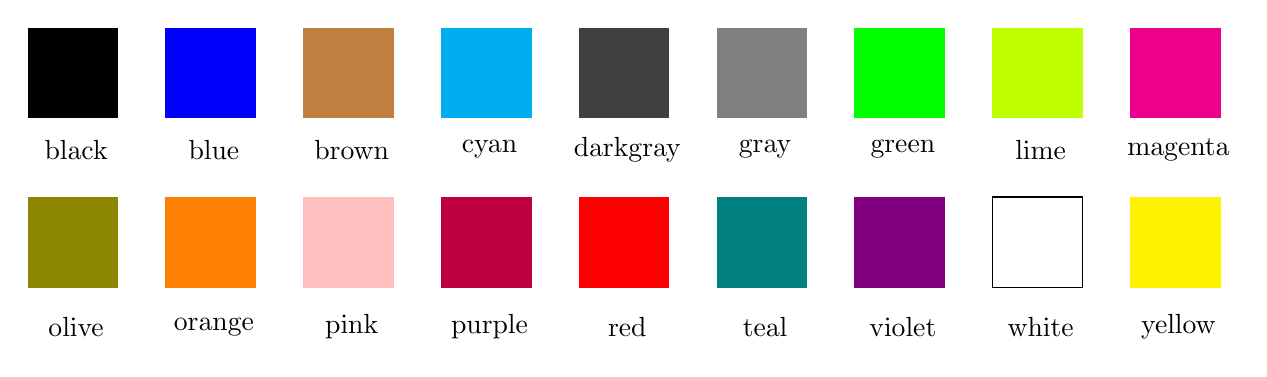
\begin{tikzpicture}
\fill [black] (0,0) rectangle ++(1.15,1.15);
\draw (0.615,-0.4) node {black};
\fill [blue] (1.75,0) rectangle ++(1.15,1.15);
\draw (2.365,-0.4) node {blue};
\fill [brown] (3.5,0) rectangle ++(1.15,1.15);
\draw (4.115,-0.4) node {brown};
\fill [cyan] (5.25,0) rectangle ++(1.15,1.15);
\draw (5.865,-0.4) node {cyan};
\fill [darkgray] (7,0) rectangle ++(1.15,1.15);
\draw (7.615,-0.4) node {darkgray};
\fill [gray] (8.75,0) rectangle ++(1.15,1.15);
\draw (9.365,-0.4) node {gray};
\fill [green] (10.5,0) rectangle ++(1.15,1.15);
\draw (11.115,-0.4) node {green};
\fill [lime] (12.25,0) rectangle ++(1.15,1.15);
\draw (12.865,-0.4) node {lime};
\fill [magenta] (14,0) rectangle ++(1.15,1.15);
\draw (14.615,-0.4) node {magenta};

\fill [olive] (0,-1) rectangle ++(1.15,-1.15);
\draw (0.615,-2.65) node {olive};
\fill [orange] (1.75,-1) rectangle ++(1.15,-1.15);
\draw (2.365,-2.65) node {orange};
\fill [pink] (3.5,-1) rectangle ++(1.15,-1.15);
\draw (4.115,-2.65) node {pink};
\fill [purple] (5.25,-1) rectangle ++(1.15,-1.15);
\draw (5.865,-2.65) node {purple};
\fill [red] (7,-1) rectangle ++(1.15,-1.15);
\draw (7.615,-2.65) node {red};
\fill [teal] (8.75,-1) rectangle ++(1.15,-1.15);
\draw (9.365,-2.65) node {teal};
\fill [violet] (10.5,-1) rectangle ++(1.15,-1.15);
\draw (11.115,-2.65) node {violet};
\draw[fill=white] (12.25,-1) rectangle ++(1.15,-1.15);
\draw (12.865,-2.65) node {white};
\fill [yellow] (14,-1) rectangle ++(1.15,-1.15);
\draw (14.615,-2.65) node {yellow};
\end{tikzpicture}
%%\end{texexptitled}
\end{center}

Assim como em qualquer editor de textos WYSIWYG, as cores do texto podem ser alteradas para palavras isoladas, frases ou parágrafos.

\begin{texexptitled}[breakable,center lower,enhanced,middle=2mm]{Texto com fonte colorida}{exe_cor1}
\textit{The \color{pink}{quick} \color{magenta}{brown} fox jumps \color{green}{over} the lazy \color{blue}{dog}.}
\end{texexptitled}

Além de modificar a cor das fontes, é possível também marcá-las de forma que o fundo fique colorido.

\begin{texexptitled}[breakable,center lower,enhanced,middle=2mm]{Texto com fundo colorido}{exe_cor3}
\textit{The \colorbox{pink}{quick} \colorbox{magenta}{brown} fox jumps \colorbox{green}{over} the lazy \colorbox{blue}{dog}.}
\end{texexptitled}

Você pode escolher, por exemplo, utilizar a patela de cores do projeto ``Solarized''. Para utilizá-la, basta carregar o pacote \mintinline{latex}{\usepackage{solarized}}. A paleta de cores do ``Solarized'' é a seguinte:

%\begin{center}
%\solarizedPalette
%\end{center}

\begin{center}
\begin{tikzpicture}
\fill [solarized-base03] (0,0) rectangle ++(1.15,1.15);
\draw (0.615,-0.4) node {base03};
\fill [solarized-base02] (1.75,0) rectangle ++(1.15,1.15);
\draw (2.365,-0.4) node {base02};
\fill [solarized-base01] (3.5,0) rectangle ++(1.15,1.15);
\draw (4.115,-0.4) node {base01};
\fill [solarized-base00] (5.25,0) rectangle ++(1.15,1.15);
\draw (5.865,-0.4) node {base00};
\fill [solarized-base0] (7,0) rectangle ++(1.15,1.15);
\draw (7.615,-0.4) node {base0};
\fill [solarized-base1] (8.75,0) rectangle ++(1.15,1.15);
\draw (9.365,-0.4) node {base1};
\fill [solarized-base2] (10.5,0) rectangle ++(1.15,1.15);
\draw (11.115,-0.4) node {base2};
\fill [solarized-base3] (12.25,0) rectangle ++(1.15,1.15);
\draw (12.865,-0.4) node {base3};
%\fill [solarized-] (14,0) rectangle ++(1.15,1.15);
%\draw (14.615,-0.4) node {teal};

\fill [solarized-yellow] (0,-1) rectangle ++(1.15,-1.15);
\draw (0.615,-2.65) node {yellow};
\fill [solarized-orange] (1.75,-1) rectangle ++(1.15,-1.15);
\draw (2.365,-2.65) node {orange};
\fill [solarized-red] (3.5,-1) rectangle ++(1.15,-1.15);
\draw (4.115,-2.65) node {red};
\fill [solarized-magenta] (5.25,-1) rectangle ++(1.15,-1.15);
\draw (5.865,-2.65) node {magenta};
\fill [solarized-violet] (7,-1) rectangle ++(1.15,-1.15);
\draw (7.615,-2.65) node {violet};
\fill [solarized-blue] (8.75,-1) rectangle ++(1.15,-1.15);
\draw (9.365,-2.65) node {blue};
\fill [solarized-cyan] (10.5,-1) rectangle ++(1.15,-1.15);
\draw (11.115,-2.65) node {cyan};
\fill [solarized-green] (12.25,-1) rectangle ++(1.15,-1.15);
\draw (12.865,-2.65) node {green};
%\fill [solarized-] (14,-1) rectangle ++(1.15,-1.15);
%\draw (14.615,-2.65) node {grey};
\end{tikzpicture}
\end{center}

Para utilizar as novas cores, basta utilizar um dos nomes definidos pela paleta, precedido por \mintinline{latex}{solarized-}. Por exemplo: \mintinline{latex}{solarized-red}.

Outra paleta de cores armoniozas, é provido pelo pacote {\tt xcolor-material}. Esta é a paleta de cores do \textit{Material Design} do Google. Para utilizá-la, basta carregar o pacote \mintinline{latex}{\usepackage{xcolor-material}} no preâmbulo do documento. 

As cores básicas do pacote {xcolor-material} são as seguintes (além do branco e preto):

\begin{center}
\begin{tikzpicture}
\fill [MaterialRed] (0,0) rectangle ++(1.15,1.15);
\draw (0.615,-0.4) node {red};
\fill [MaterialPink] (1.75,0) rectangle ++(1.15,1.15);
\draw (2.365,-0.4) node {pink};
\fill [MaterialPurple] (3.5,0) rectangle ++(1.15,1.15);
\draw (4.115,-0.4) node {purple};
\fill [MaterialDeepPurple] (5.25,0) rectangle ++(1.15,1.15);
\draw (5.865,-0.4) node {d. purple};
\fill [MaterialIndigo] (7,0) rectangle ++(1.15,1.15);
\draw (7.615,-0.4) node {indigo};
\fill [MaterialBlue] (8.75,0) rectangle ++(1.15,1.15);
\draw (9.365,-0.4) node {blue};
\fill [MaterialLightBlue] (10.5,0) rectangle ++(1.15,1.15);
\draw (11.115,-0.4) node {l. blue};
\fill [MaterialCyan] (12.25,0) rectangle ++(1.15,1.15);
\draw (12.865,-0.4) node {cyan};
\fill [MaterialTeal] (14,0) rectangle ++(1.15,1.15);
\draw (14.615,-0.4) node {teal};

\fill [MaterialGreen] (0,-1) rectangle ++(1.15,-1.15);
\draw (0.615,-2.65) node {green};
\fill [MaterialLightGreen] (1.75,-1) rectangle ++(1.15,-1.15);
\draw (2.365,-2.65) node {l. green};
\fill [MaterialLime] (3.5,-1) rectangle ++(1.15,-1.15);
\draw (4.115,-2.65) node {lime};
\fill [MaterialYellow] (5.25,-1) rectangle ++(1.15,-1.15);
\draw (5.865,-2.65) node {yellow};
\fill [MaterialAmber] (7,-1) rectangle ++(1.15,-1.15);
\draw (7.615,-2.65) node {amber};
\fill [MaterialOrange] (8.75,-1) rectangle ++(1.15,-1.15);
\draw (9.365,-2.65) node {orange};
\fill [MaterialDeepOrange] (10.5,-1) rectangle ++(1.15,-1.15);
\draw (11.115,-2.65) node {d. orange};
\fill [MaterialBrown] (12.25,-1) rectangle ++(1.15,-1.15);
\draw (12.865,-2.65) node {brown};
\fill [MaterialGrey] (14,-1) rectangle ++(1.15,-1.15);
\draw (14.615,-2.65) node {grey};
\end{tikzpicture}
\end{center}

Na paleta de cores mostrada acima, ``d.'' foi utilizado para abreviar a palavra \textit{deep} e ``l.'' foi utilizada para abreviar a palavra \textit{light}. Para utilizar as cores do pacote {\tt xcolor-material}, é necessário utilizá-las da seguinte forma: a cor \textit{Deep Purple} deve ser referenciada como ``MaterialDeepPurple'', ou seja, a palavra reservada ``Material'' deve preceder o nome da cor, que por sua vez, deve ser indicada com a primeira letra em caixa alta.

\begin{marker}
  Pode ser necessário incluir o arquivo {\tt xcolor-material.sty} à sua distribuição LaTeX. Veja a página do pacote para mais informações (\url{https://www.ctan.org/pkg/xcolor-material}).
\end{marker}

Se for necessário, é possível definir qualquer cor utilizando códigos HTML, \textit{Red Green Blue} (RGB) ou \textit{Cyan Magenta Yellow Black} (CMYK) utilizando o comando \mintinline{latex}{\definecolor}.

\begin{texexptitled}[breakable,center lower,enhanced,middle=2mm]{Definindo cores}{exe_cor4}
\definecolor{meularanja1}{HTML}{FF7F00}
\definecolor{meularanja2}{rgb}{1,0.5,0}
\definecolor{meularanja3}{RGB}{255,127,0}
\definecolor{meularanja4}{cmyk}{0,0.5,1,0}


\begin{tikzpicture}
\fill [meularanja1] (0,0) rectangle ++(1.25,1.25);
\draw (0.6,-0.5) node {meularanja1};
\fill [meularanja2] (3,0) rectangle ++(1.25,1.25);
\draw (3.6,-0.5) node {meularanja2};
\fill [meularanja3] (6,0) rectangle ++(1.25,1.25);
\draw (6.6,-0.5) node {meularanja3};
\fill [meularanja4] (9,0) rectangle ++(1.25,1.25);
\draw (9.6,-0.5) node {meularanja4};
\end{tikzpicture}
\end{texexptitled}

\begin{marker}
Veja outras opções de paletas e cores em \href{http://latexcolor.com}{LaTeXColor}.
\end{marker}

\subsection{Medidas}
\label{sec:medidas}

As medidas na linguagem LaTeX podem ser apresentadas em unidades diversas. Você pode misturá-las e isso pode ocorrer quando você reutiliza algum código que produz uma formatação específica que você gostaria de criar e acabou encontrando na internet. A Tabela \ref{tab:medidas} a seguir, mostra as unidades mais comuns. Vale ressaltar, entretanto, que a unidade padrão é o ponto e que o comprimento padrão é \mintinline{latex}{1 pt}:

\begin{table}[H]
\centering
\caption{Unidades de Medidas mais Comuns no LaTeX.}
\label{tab:medidas}
%\begin{center}
    \begin{tabular}{p{3cm}c{3cm}c{5cm}}
    \hline
    \\[-0.5em]
    \textbf{Abreviação} & \textbf{Definição} & \textbf{Valor em Pontos} \\
    \\[-0.5em]
    \hline
    \hline
    \\[-0.5em]
    Ponto           & \mintinline{latex}{pt} & $1$                              \\
    \\[-0.5em]
    Milímetro       & \mintinline{latex}{mm} & $2,84$ = $\frac{7227}{2540}$     \\
    \\[-0.5em]
    Centímetro      & \mintinline{latex}{cm} & $28,4$ = $\frac{7227}{254}$      \\
    \\[-0.5em]
    Polegada        & \mintinline{latex}{in} & $72,27$     \\
    \\[-0.5em]
    Altura de ``x'' & \mintinline{latex}{ex} & \textit{Depende da fonte utilizada} \\
    \\[-0.5em]
    Altura de ``M'' & \mintinline{latex}{em} & \textit{Depende da fonte utilizada} \\
    \\[-0.5em]
    \hline
    \end{tabular}
%\end{center}
%\label{tab:medidas}
\end{table}

Em documentos escritos na linguagem LaTeX, é possível especificar as medidas utilizando os valores nas unidades indicadas na tabela acima e também utilizando algumas macros. Estas macros são, especificamente, representam algumas medidas padrão na linguagem e são apresentadas na Tabela \ref{tab:meds_padrao} abaixo.

\begin{table}[H]
\centering
\caption{Algumas Macros de Medidas do LaTeX.}
\label{tab:meds_padrao}
%\begin{center}
    \begin{tabular}{p{5cm}p{8cm}}
    \hline
    \\[-0.5em]
    \textbf{Macro} & \textbf{Descrição} \\
    \\[-0.5em]
    \hline
    \hline
    \\[-0.5em]
    \mintinline{latex}{\baselineskip}    & Distância vertical entre as linhas em um parágrafo \\
    \\[-0.5em]
    \mintinline{latex}{\baselinestretch} & Fator para ser utilizado com o marcador \mintinline{latex}{\baselineskip} (exemplo: \mintinline{latex}{\renewcommand{\baselinestretch}{fator}}) \\
    \\[-0.5em]
    \mintinline{latex}{\columnsep}       & Distância entre colunas \\
    \\[-0.5em]
    \mintinline{latex}{\columnwidth}     &  Largura de uma coluna \\
    \\[-0.5em]
    \mintinline{latex}{\evensidemargin}  & Margens em páginas `pares' \\
    \\[-0.5em]
    \mintinline{latex}{\linewidth}       & Largura de uma linha em um ambiente local \\
    \\[-0.5em]
    \mintinline{latex}{\oddsidemargin}   & Margens em páginas `ímpares' \\
    \\[-0.5em]
    \mintinline{latex}{\paperwidth}      & Largura de uma página \\
    \\[-0.5em]
    \mintinline{latex}{\paperheight}     & Altura de uma página \\
    \\[-0.5em]
    \mintinline{latex}{\parindent}       & Identação de um parágrafo \\
    \\[-0.5em]
    \mintinline{latex}{\parskip}         & Espaçamento extra entre parágrafos \\
    \\[-0.5em]
    \mintinline{latex}{\tabcolsep}       & Separação normal entre as colunas no ambiente \mintinline{latex}{\tabular} \\
    \\[-0.5em]
    \mintinline{latex}{\textheight}      & Altura do texto na página \\
    \\[-0.5em]
    \mintinline{latex}{\textwidth}       & Largura do texto na página \\
    \\[-0.5em]
    \mintinline{latex}{\topmargin}       & Tamanho da margem de cima \\
    \\[-0.5em]
    \mintinline{latex}{\unitlength}      & Unidades de comprimento no ambiente \mintinline{latex}{\picture} \\
    \\[-0.5em]
    \hline
    \end{tabular}
%\end{center}
%\label{tab:medidas}
\end{table}

No LaTeX, um comprimento é um número real seguido por uma unidade de media, o qual pode ser modificado por um valor ou uma macro. 

%% INCLUIR ALGUNS EXEMPLOS DE USO DOS COMANDOS DA TABELA ACIMA.

%\begin{texexptitled}{Comprimento modificado por um valor \mintinline{latex}{50.5pt plus 1pt minus 2pt}}{exe_medidas1}
%\setlength{\parindent}{0em}
%\lipsum[1]
%\setlength{\parindent}{50.5pt plus 1pt minus 2pt}
%\lipsum[2]
%\end{texexptitled}
%
%\begin{texexptitled}{Comprimento modificado por uma macro \mintinline{latex}{10\textwidth}}{exe_medidas2}
%\setlength{\parindent}{0em}
%\lipsum[1]
%\setlength{\parindent}{10\textwidth}
%\lipsum[2]
%\end{texexptitled}

\begin{marker}
Veja mais detalhes, informações e exemplos em \url{https://en.wikibooks.org/wiki/LaTeX/Lengths}.
\end{marker}

\subsection{Parágrafos}
\label{sec:paragrafos}

Os parágrafos no LaTeX são blocos de texto separados por uma ou mais linhas. Para iniciar um parágrafo, basta pular uma linha. Uma outra forma de separar parágrafos, é através da utilização de duas barras invertidas (\mintinline{latex}{\\}). Observe as diferenças entre os exemplos a seguir.

\begin{texexptitled}[breakable,enhanced,middle=2mm]{Parágrafos Contíguos}{exe_par1}
\lipsumsentence[1-4] 
\lipsumsentence[5-8]
\end{texexptitled}

\begin{texexptitled}[breakable,enhanced,middle=2mm]{Parágrafos Separados por um Espaço}{exe_par2}
\lipsumsentence[1-4]  

\lipsumsentence[5-8]
\end{texexptitled}

\begin{texexptitled}[breakable,enhanced,middle=2mm]{Parágrafos Separados por Duas Barras invertidas (\mintinline{latex}{\\})}{exe_par3}
\lipsumsentence[1-4] \\ 
\lipsumsentence[5-8]
\end{texexptitled}

\subsubsection*{Posição e espaçamento}
\label{sec:pos_espac}

Boa parte dos elementos de um texto podem ser, basicamente, posicionados à esquerda, ao centro ou à direita. O LaTeX possui marcadores especiais para estes posicionamentos, que podem ser utilizados não apenas nos parágrafos, mas também com figuras e tabelas.

\begin{texexptitled}[breakable,enhanced,middle=2mm]{Parágrafos centralizados \par Utilizando o ambiente \mintinline{latex}{center}}{exe_par4}
\begin{center}
\lipsumsentence[9-10] \\ 
\lipsumsentence[11-12]
\end{center}
\end{texexptitled}

Além de utilizar o ambiente \mintinline{latex}{center}, é possível utilizar o marcador \mintinline{latex}{\centering}.

\begin{texexptitled}[breakable,enhanced,middle=2mm]{Parágrafos centralizados \par Utilizando o marcador \mintinline{latex}{\centering}}{exe_par5}
\centering
\lipsumsentence[13-14] \\ 
\lipsumsentence[15-16]
\end{texexptitled}

\begin{texexptitled}[breakable,enhanced,middle=2mm]{Parágrafos alinhados à esquerda}{exe_par6}
\begin{flushleft}
\lipsumsentence[17-18] \\ 
\lipsumsentence[19-20]
\end{flushleft}
\end{texexptitled}

\begin{texexptitled}[breakable,enhanced,middle=2mm]{Parágrafos alinhados à direita}{exe_par7}
\begin{flushright}
\lipsumsentence[21-22] \\ 
\lipsumsentence[23-24]
\end{flushright}
\end{texexptitled}

Espaçamentos horizontais e verticais são dados pelos marcadores \mintinline{latex}{\vspace{}} e \mintinline{latex}{\hspace{}}, respectivamente.

% Ver mais em: https://tex.stackexchange.com/questions/30062/vspace-vs-vskip

\begin{texexptitled}[breakable,enhanced,middle=2mm]{Espaçamento vertical}{exe_par8}
\lipsumsentence[21-22] 
\vspace{1cm}
\lipsumsentence[23-27]
\end{texexptitled}

\begin{texexptitled}[breakable,enhanced,middle=2mm]{Espaçamento horizontal}{exe_par9}
\hspace{2cm}\lipsumsentence[28-29] \\ 
\lipsumsentence[30-31]
\end{texexptitled}

%\subsection{Espaçamentos e quebras de linhas}
%\subsection{Ambientes (center, flushleft, flushright) (itemize, description, enumerate)}

%\subsubsection*{Índices e expoentes}
%\label{sec:ind_exps}

\subsubsection*{Notas de rodapé}
\label{sec:notas_rodape}

Notas de rodapé podem ser inseridas com o marcador \mintinline{latex}{\footnote{}} após a palavra a qual se quer referir. Nos exemplos a seguir, vamos usar o pangrama\footnotemark{} ``\textit{À noite, vovô Kowalsky vê o ímã cair no pé do pinguim queixoso e vovó põe açúcar no chá de tâmaras do jabuti feliz\footnotemark{}}''. O Exemplo \ref{exe_rodape1} mostra como utilizar o marcador \mintinline{latex}{\footnote{}}:

\begin{texexptitled}[breakable,enhanced,middle=2mm]{Nota de rodapé utilizando o marcador \mintinline{latex}{\footnote}}{exe_rodape1}
À noite, vovô Kowalsky\footnote{Esta é uma nota de rodapé.} vê o ímã cair no pé do pinguim queixoso e vovó põe açúcar no chá de tâmaras do jabuti feliz\footnote{Este é uma outra nota de rodapé}.
\end{texexptitled}

\addtocounter{footnote}{-2}
\stepcounter{footnote}\footnotetext{Um pangrama é uma sentença que possui todas as letras do alfabeto.}
\stepcounter{footnote}\footnotetext{Este pangrama contém 90 caracteres e todas as letras acentuadas: à, á, â, é, ê, í, ó, ô, õ, ú e ç.}

No Exemplo \ref{exe_rodape1}, foram incluídas duas notas de rodapé. Elas são ordenadas sequencialmente ao final da página em que foram inseridas.

Outra forma de incluir notas de rodapé, é a partir da utilização dos marcadores \mintinline{latex}{\footnotemark} e \mintinline{latex}{\footnotetext}. O primeiro, insere o marcador na posição desejada, e o segundo, insere o texto referente àquele marcador. Esta forma é mais clara, pois destacam-se os comandos e marcadores fora do parágrafo que se está escrevendo, deixando-o mais limpo. Veja o Exemplo \ref{exe_rodape2} a seguir:

\begin{texexptitled}[breakable,enhanced,middle=2mm]{Nota de rodapé utilizando os marcadores \mintinline{latex}{\footnotemark} e \minitable{latex}{\footnotetext}}{exe_rodape2}
À noite, vovô Kowalsky vê o ímã\footnotemark{} cair no pé do pinguim queixoso\footnotemark{} e vovó põe açúcar no chá de tâmaras do jabuti feliz.

\footnotetext{Esta é uma nota de rodapé.}
\footnotetext{Esta é uma outra nota de rodapé.}
\end{texexptitled}

Um problema bastante comum com notas de rodapé no LaTeX ao se utilizar os marcadores \mintinline{latex}{\footenotemark} e \mintinline{latex}{\footnotetext}, é que os índices de marcação podem se repetir nas notas de rodapé. Veja no Exemplo \ref{exe_rodape3}:

\begin{texexptitled}[breakable,enhanced,middle=2mm]{Nota de rodapé utilizando o marcado \mintinline{latex}{\footnote}}{exe_rodape3}
À noite, vovô Kowalsky\footnote{Esta é uma nota de rodapé.} vê o ímã cair no pé do pinguim queixoso e vovó põe açúcar no chá de tâmaras do jabuti feliz\footnote{Este é uma outra nota de rodapé}.
\end{texexptitled}

%\begin{texexptitled}[breakable,enhanced,middle=2mm]{Nota de rodapé utilizando o marcado \mintinline{latex}{\footnote{}}}{exe_rodape1}
%À noite, vovô Kowalsky\footnote{Esta é uma nota de rodapé.} vê o ímã cair no pé do pinguim queixoso e vovó põe açúcar no chá de tâmaras do jabuti feliz\footnote{Este é uma outra nota de rodapé}.
%\end{texexptitled}

No Exemplo \ref{exe_rodape1}, observe que o estilo aplicado à nota de rodapé é alfabético. É possível alterar o estilo de numeração renovando o marcador {\tt footnote}, e.g, \mintinline{latex}{\renewcommand{\thefootnote}{\roman{footnote}}}. Neste caso, a opção {\tt roman} indica que o estilo de numeração dos índices dos marcadores será em algarismos romanos:

\renewcommand{\thefootnote}{\roman{footnote}}

\begin{texexptitled}[breakable,enhanced,middle=2mm]{Nota de rodapé com referência numérica}{exe_rodape4}
À noite, vovô Kowalsky vê o ímã\footnotemark{} cair no pé do pinguim queixoso\footnotemark{} e vovó põe açúcar\footnote{Esta é mais uma nota de rodapé} no chá de tâmaras do jabuti feliz.

\footnotetext{Esta é uma nota de rodapé.}
\footnotetext{Esta é uma outra nota de rodapé.}
\end{texexptitled}

\subsubsection*{Listas}
\label{sec:listas}

Listas ordenadas e não ordenadas podem ser facilmente criadas no LaTeX dentro de ambientes específicos. Listas não ordenadas são criadas dentro do ambiente \mintinline{latex}{itemize} e listas ordenadas são criadas dentro do ambiente \mintinline{latex}{enumerate}.

No Exemplo \ref{exe_lista1}, tem-se uma lista simples não ordenada.

\begin{texexptitled}[breakable,enhanced,middle=2mm]{Lista não ordenada utilizando o ambiente \mintinline{latex}{itemize}}{exe_lista1}
\begin{itemize}
    \item Item 1
    \item Item 2
    \item Item 3
\end{itemize}
\end{texexptitled}

Listas podem ser aninhadas, de forma que subitens possam ser obtidos. Observe no Exemplo \ref{exe_lista2} que o estilo dos subitens é alterado automaticamente:

\begin{texexptitled}[breakable,enhanced,middle=2mm]{Lista não ordenada aninhada utilizando o ambiente \mintinline{latex}{itemize}}{exe_lista2}
\begin{itemize}
    \item Item 1
    \begin{itemize}
        \item Item 1.1
        \item Item 1.2
    \end{itemize}
    \item Item 2
    \item Item 3
    \begin{itemize}
        \item Item 3.1
        \item Item 3.2
        \item Item 3.3
    \end{itemize}
\end{itemize}
\end{texexptitled}

No Exemplo \ref{exe_lista3} a seguir, tem-se uma lista simples ordenada. Compare com o Exemplo \ref{exe_lista1} e veja a única diferença entre eles está apenas no tipo de ambiente utilizado ({\tt itemize} e {\tt enumerate}, respectivamente).

\begin{texexptitled}[breakable,enhanced,middle=2mm]{Lista ordenada utilizando o ambiente \mintinline{latex}{enumerate}}{exe_lista3}
\begin{enumerate}
    \item Item 1
    \item Item 2
    \item Item 3
\end{enumerate}
\end{texexptitled}

Assim como nas listas não ordenadas, listas ordenadas também podem ser aninhadas. Neste caso, observe que a numeração dos subitens é incrementada automaticamente:

\begin{texexptitled}[breakable,enhanced,middle=2mm]{Lista ordenada aninhada utilizando o ambiente \mintinline{latex}{enumerate}}{exe_lista4}
\begin{enumerate}
    \item Item 1
    \begin{enumerate}
        \item Item 1.1
        \begin{enumerate}
            \item Item 1.1.1
            \item Item 1.1.2
        \end{enumerate}
        \item Item 1.2
    \end{enumerate}
    \item Item 2
    \item Item 3
    \begin{enumerate}
        \item Item 3.1
         \begin{enumerate}
            \item Item 3.1.1
            \begin{enumerate}
                \item Item 3.1.1.1
                \item Item 3.1.1.2
            \end{enumerate}
            \item Item 3.1.2
        \end{enumerate}
        \item Item 3.2
    \end{enumerate}
\end{enumerate}
\end{texexptitled}

Listas ordenadas podem ser organizadas de formas diferentes. Pode-se organizadas de forma numérica, alfabética ou de forma alfanumérica. Para alterar a forma como as listas são ordenadas, é necessário definir o estilo de ordenamento com o comando \mintinline{latex}{labelenum<nível>}{<estilo>}, onde {\tt <nível>} pode ser {\tt i}, {\tt ii}, {\tt iii} ou {\tt vi}. O estilo, dado pelo modificador {\tt <estilo>}, pode assumir as seguintes opções:

\begin{enumerate}
    \item {\tt alph} Letras minúsculas (a, b, c, ...);
    \item {\tt Alph} Letras maiúsculas (A, B, C, ...);
    \item {\tt arabic} Numerais arábicos (1, 2, 3, ...);
    \item {\tt roman} Numerais minúsculos romanos (i, ii, iii, ...);
    \item {\tt Roman} Numerais maiúsculos romanos (I, II, III, ...).
\end{enumerate}

Combinando os estilos listados acima com os níveis, o comando \mintinline{latex}{labelenum<nível>}{<estilo>} pode assumir algumas das seguintes construções:

\begin{itemize}
    \item Numerais arábicos (1, 2, 3, ...) no Nível 1:\\
    \mintinline{latex}{\renewcommand{\labelenumi}{\arabic{enumi}}}
    \item Letras minúsculas (a, b, c, ...) no Nível 2:\\ \mintinline{latex}{\renewcommand{\labelenumii}{\alph{enumii}}}
    \item Numerais minúsculos romanos (i, ii, iii, ...) no Nível 3:\\ \mintinline{latex}{\renewcommand{\labelenumiii}{\roman{enumiii}}}
    \item Letras maiúsculas (A, B, C, ...) no Nível 4:\\ \mintinline{latex}{\renewcommand{\labelenumiv}{\Alph{enumiv}}}
\end{itemize}

No Exemplo \ref{exe_lista5} a seguir, alteramos o estilo de ordenamento do Nível 2, utilizando algarismos romanos:

\begin{texexptitled}[breakable,enhanced,middle=2mm]{Lista ordenada aninhada com níveis customizados}{exe_lista5}
\renewcommand{\labelenumi}{\arabic{enumi}}
\renewcommand{\labelenumii}{\alph{enumii}}
\renewcommand{\labelenumiii}{\roman{enumiii}}
\renewcommand{\labelenumiv}{\Alph{enumiv}}
\begin{enumerate}
    \item Item 1
    \begin{enumerate}
        \item Item 1.1
        \begin{enumerate}
            \item Item 1.1.1
            \item Item 1.1.2
        \end{enumerate}
        \item Item 1.2
    \end{enumerate}
    \item Item 2
    \item Item 3
    \begin{enumerate}
        \item Item 3.1
         \begin{enumerate}
            \item Item 3.1.1
            \begin{enumerate}
                \item Item 3.1.1.1
                \item Item 3.1.1.2
            \end{enumerate}
            \item Item 3.1.2
        \end{enumerate}
        \item Item 3.2
    \end{enumerate}
\end{enumerate}
\end{texexptitled}


\subsection{Figuras}% (ambientes figure e subfigure)}
\label{sec:figuras}

Figuras podem ser incluídas em um documento LaTeX de formas variadas. Dependendo da complexidade da informação apresentada, ambientes específicos devem ser utilizados para organizar não apenas a apresentação, mas também a redação do documento.

Uma figura pode ser incluída de forma simples utilizando o marcador \mintinline{latex}{\includegraphics[]{}}.

% Ref: https://tex.stackexchange.com/questions/231738/example-images-in-latex
\begin{texexptitled}[breakable,enhanced,middle=2mm]{Figura com o marcador \mintinline{latex}{\includegraphics[]{}}}{exe_fig1}
\includegraphics[width=3cm]{example-image-a}
\includegraphics[width=3cm]{example-image-golden}
\includegraphics[width=3cm]{example-grid-100x100pt}
\includegraphics[height=5cm]{example-image-b} 
\includegraphics[scale=0.5]{example-image-c} 
\includegraphics[width=3cm]{example-image} 
\end{texexptitled}

\begin{marker}
  As imagens do Exemplo \ref{exe_fig1} acima foram incluídas com o pacote \mintinline{latex}{graphicsx} que possui diversas imagens de exemplos.
\end{marker}

No Exemplo \ref{exe_fig1}, observe que o marcador \mintinline{latex}{\includegraphics} aceita algumas opções que são delimitadas por um par de $[]$'s. Pode-se especificar, por exemplo, o tamanho da figura pode ser especificado com as opções \mintinline{latex}{width}, \mintinline{latex}{height} ou \mintinline{latex}{scale}.

\subsection{Formatos de Figuras}
\label{sec:form_figs}

Figuras podem ser incorporadas a partir de diferentes formatos em um documento LaTeX. Os formatos preferenciais, entretanto, são o PDF e o EPS. Estes formatos são vetoriais e permitem, por exemplo, a impressão em alta resolução das figuras.

É possível converter formatos como o PNG, GIF e JPEG para os formatos PDF e EPS. Para tanto, recomenda-se a utilização do programa \textit{Imagemagick} para esta conversão. Conversores online também podem ser utiizados para esta finalidade.

O \textit{Imagemagick} possui um \textit{script} chamado \textit{convert} que pode ser utilizado para realizar a conversão entre estes formatos:

\begin{commandshell}
for i in \$(ls *.png); do j=\$(echo \$i | sed 's,.png,.pdf,g'); convert -i \$i -o\$j; done
\end{commandshell}

Outro detalhe que pode ser importante, é remover os espaços em branco nas margens das figuras. Isso é útil especialmente quando deseja-se incluir figuras lado a lado. Para isso, pode-se utilizar o \textit{script} \href{http://www.fmwconcepts.com/imagemagick/autotrim/index.php}{\textit{autotrim}} (que utiliza o comando \textit{convert}):

\begin{commandshell}
autotrim -i figura.png -o figura_crop.png
\end{commandshell}

\begin{marker}
Veja a página \url{http://www.fmwconcepts.com/imagemagick/index.php} com diversos exemplos e \textit{scripts} úteis do \textit{Imagemagick}.
\end{marker}

\begin{marker}
  Para mais exemplos sobre a incorporação e conversão entre formatos de arquivos de imagens, tenha como referência a página \url{https://en.wikibooks.org/wiki/LaTeX/Importing_Graphics}.
\end{marker}

%\subsection{Construção de diagramas e outras figuras (tickz)}
\subsubsection*{Ambientes de figuras}
\label{sec:amb_figs}

A forma mais simples de incluir figuras em um documento LaTeX, é a partir do comando \mintinline{latex}{\includegraphics[]{}}. Observe que este comando (assim como a maioria dos comandos e marcadores da linguagem) possui uma seção de opções (ou argumentos) que são indicados entre os colchetes e o caminho para a imagem em si, que é informada entre as chaves. O Exemplo \ref{exe_incgraphs} mostra um exemplo simples:

\begin{texexptitled}[breakable,enhanced,middle=2mm]{Incorporando uma figura com o comando \mintinline{latex}{\includegraphics[]{}}}{exe_incgraphs}
\includegraphics[width=3cm]{example-image-a}
\end{texexptitled}

Observe, entretando, que apenas inserimos uma figura, mas não definimos uma posição relativa ao parágrafo ou à página. Para isso, é necessário incorporar o comando \mintinline{latex}{\includegraphics[]{}} dentro de um ambiente específico que permita o seu posicionamento relativo. Este ambiente, é o ambiente {\tt figure}. O Exemplo \ref{exe_ambfig} mostra um exemplo com o ambiente {\tt figure}:

\begin{texexptitled}[breakable,enhanced,middle=2mm]{Incorporando uma figura com o comando \mintinline{latex}{\includegraphics[]{}} dentro do ambiente {\tt figure}}{exe_ambfig}
\begin{figure}[h]
\includegraphics[width=3cm]{example-image-a}
\end{figure}
\end{texexptitled}

O ambiente {\tt figure} deve ser configurado para possuir uma das seguintes posições relativas:

% FONTE: https://www.overleaf.com/learn/latex/Inserting_Images
\begin{table}[H]
\centering
\caption{Opções de posicionamento relativo do ambiente {\tt figure}.}
\label{tab:ambfig}
%\begin{center}
    \begin{tabular}{p{2cm}p{11cm}}
    \hline
    \\[-0.5em]
    \textbf{Opção} & \textbf{Descrição} \\
    \\[-0.5em]
    \hline
    \hline
    \\[-0.5em]
    {\tt h} & Posiciona o ambiente ``aqui'' ({\tt h} vem do inglês \textit{here}). A posição exata pode variar dependendo dos outros elementos textuais \\
    \\[-0.5em]
    {\tt t} & Posiciona o ambiente no ``topo'' da página ({\tt t} vem do inglês \textit{top}) \\
    \\[-0.5em]
    {\tt b} & Posiciona o ambiente na ``base'' da página ({\tt b} vem do inglês \textit{bottom}) \\
    \\[-0.5em]
    {\tt p} & Posiciona o ambiente em uma ``página'' separada ({\tt p} vem do inglês \textit{page}) \\
    \\[-0.5em]
    {\tt !} & Força o LaTeX a usar a posição textual onde o ambiente se encontra (e.g., {\tt h!}) \\
    \\[-0.5em]
    {\tt H} & Posiciona o ambiente precisamente no local em que se encontra (depende do pacote {\tt float} e é equivalente a {\tt h!}) \\
    \\[-0.5em]
    \hline
    \end{tabular}
%\end{center}
%\label{tab:medidas}
\end{table}

No Exemplo \ref{exe_ambfig_H} é mostrado o posicionamento de uma figura utilizando a posição relativa {\tt H}:

\begin{texexptitled}[breakable,enhanced,middle=2mm]{Incorporando uma figura com o comando \mintinline{latex}{\includegraphics[]{}} dentro do ambiente {\tt figure} com a posição relativa {\tt H}}{exe_ambfig_H}
\lipsum[1]
\begin{figure}[H]
\includegraphics[width=3cm]{example-image-a}
\end{figure}
\lipsum[2]
\end{texexptitled}

\begin{marker}
  No estilo do INPE, o ambiente padrão para o posicionamento do ambiente {\tt figure} é {\tt H}.
\end{marker}

Uma vez definido o posicionamento relativo (i.e., relativo ao parágrafo ou página), pode-se centralizar a figura utilizando-se o marcador \mintinline{latex}{\centering} ou o ambiente {\tt center}. O Exemplo \ref{exe_ambfig_center} mostra estas duas opções:

\begin{texexptitled}[breakable,enhanced,middle=2mm]{Centralizando figuras dentro do ambiente {\tt figure}}{exe_ambfig_center}
\lipsum[1]
\begin{figure}[H]
\centering
\includegraphics[width=3cm]{example-image-a}
\end{figure}
\lipsum[2]
\begin{figure}[H]
    \begin{center}
        \includegraphics[width=3cm]{example-image-a}
    \end{center}
\end{figure}
\end{texexptitled}

Observe no Exemplo \ref{exe_ambfig_center}, ambos o marcador \mintinline{latex}{\centering} e o ambiente {\tt center} devem ser colocados dentro do ambiente {\tt figure}.

Figuras podem também ser colocadas dentro de um parágrafo de forma que o texto circunde o ambiente. Para isso, é necessário utilizar o ambiente {\tt wrapfigure}:

\begin{texexptitled}[enhanced,middle=2mm]{Centralizando figuras dentro do ambiente {\tt figure}}{exe_wrapfig}
\begin{wrapfigure}{r}{0.25\textwidth}
    \centering
    \includegraphics[width=0.25\textwidth]{example-image-a}
\end{wrapfigure}
\lipsum[2]

\begin{wrapfigure}{l}{0.25\textwidth}
    \centering
    \includegraphics[width=0.25\textwidth]{example-image-b}
\end{wrapfigure}
\lipsum[3]
\end{texexptitled}

No Exemplo \ref{exe_wrapfig}, observe que o ambiente {\tt wrapfigure} aceita as opções {\tt l} e {\tt r}, que permite a figura ser alinhada à esquerda ({\tt l}, do inglês \textit{left}) ou à direita ({\tt r}, do inglês \textit{right}). Além disso, o ambiente pode ser posicionado da mesma forma como o ambiente {\tt figure} padrão.

\begin{marker}
  Consulte a página \url{https://www.overleaf.com/learn/latex/Inserting_Images} para mais opções de configuração.
\end{marker}

\subsubsection*{Construindo figuras}
\label{sec:const_figs}

%FALTA: INSERIR CODIGOS

Figuras no LaTeX podem ser desenhadas utilizando pacotes específicos. As figuras podem ser incorporadas a partir de arquivos .tex separados ou desenhadas em ambientes apropriados. O pacote TikZ é um pacote do LaTeX orientado para a construção de diagramas. Com ele você pode criar diferentes tipos de gráficos, grafos, diagramas etc, que são alinhados com o formato SVG. Com o pacote pstricks, é possível criar imagens vetoriais complexas utilizando o interpretador do \textit{GhostScript}. A diferença entre estes dois pacotes está mais relacionada com a forma como os seus resultados são interpretados e as suas imagens renderizadas dentro do documento LaTeX. %https://tex.stackexchange.com/questions/60778/fundamental-differences-pstricks-tikz-pgf-and-others

\subsubsection*{TikZ}

A Figura \ref{fig:exe_tickz} mostra um exemplo de uma imagem vetorial programada com o TickZ.

%Fonte: http://texample.net/tikz/examples/planets/
\begin{figure}[H]
\label{fig:exe_tickz}
    \begin{center}
        \resizebox{0.9\textwidth}{!}{%%%%%%%%%%%%%%%%%%%%%%%%%%%%%%%%%%%%%%%%%%%%%%%%%%%%%%%%%%%%%%%
%
% Welcome to Overleaf --- just edit your LaTeX on the left,
% and we'll compile it for you on the right. If you open the
% 'Share' menu, you can invite other users to edit at the same
% time. See www.overleaf.com/learn for more info. Enjoy!
%
%%%%%%%%%%%%%%%%%%%%%%%%%%%%%%%%%%%%%%%%%%%%%%%%%%%%%%%%%%%%%%%
% Planets
% Author: Gerard Fleuter
%\documentclass[tikz,border=10pt]{standalone}
%%%<
%\usepackage{verbatim}
%%%>
\begin{comment}
:Title: Planets
:Tags: Styles;Physics;Astronomy
:Author: Gerard Fleuter
:Slug: planets

Planets in our solar system.
\end{comment}
%\begin{document}
% definition de partial ellipse
\tikzset{partial ellipse/.style args =
  {#1:#2:#3}{insert path={+ (#1:#3) arc (#1:#2:#3)}}}
\begin{tikzpicture}[>=latex]
  %  ellipses
  \draw [fill=white!90!red]    (3,-1.8) ellipse    (4cm and 1 cm);
  \draw [fill=yellow!90!green] (3,-1.8) ellipse (3cm and 0.75 cm);
  \draw [fill=white!90!green]  (3,-1.8) ellipse  (2cm and 0.5 cm);

  % -- Soleil
  \shade [ball color=gray!10!yellow] (3,-1.8) circle (1);
  \node (soleil) at (3,-1.8) {\bf Sol};
  % partial ellipse pour tracé devant le Soleil
  \draw (3,-1.8) [partial ellipse=220:320:2cm and 0.5cm]
        (3,-1.8) [partial ellipse=220:320:3cm and 0.75cm];

  % Venus
  \shade [ball color=gray!10!orange] (1.6,-1.8) circle (.2);
  \node (venus) at (1.5,-1.45) {Vênus}; 

  % ombre de Venus
  \draw[color=white!70!black,fill=white!70!black]
    (1.6,-2.3) ellipse (2mm and 0.5mm);

  % Mercure
  \shade [ball color=gray!10!orange] (5,-1.225) circle (.25);
  \node (mercure) at (5,-0.8) {Mercúrio}; 

  % Earth
  \shade [ball color=white!50!blue] (5.75,-2.5) circle (.33);
  \node (terre) at (6.6,-2.6) {\bf Terra};

  % Lune
  \shade [ball color=yellow] (5.25,-2.8) circle (.1);
  \node (lune) at (5.25,-3) {Lua};
     
  % Mars
  \draw (3,-1.8) [partial ellipse=45:120:9cm and 2.5cm];
  \shade [ball color=black!50!red] (5,0.66) circle (.15);
  \node (mars) at (5,1) {\bf Marte};   
  % trajet
  \draw [line width=2pt,blue,->,>=latex] (terre) to[out=0,in=0] (mars);   
\end{tikzpicture}
%\end{document}}
    \end{center}
\caption{Exemplo TickZ - Planetas.}
\end{figure}

%\begin{texexptitled}{Figura com o TickZ}
%    \begin{tikzpicture}
%    \draw
%        (3,-1) coordinate (a) node[right] {a}
%        -- (0,0) coordinate (b) node[left] {b}
%        -- (2,2) coordinate (c) node[above right] {c}
%        pic["$\alpha$", draw=orange, <->, angle eccentricity=1.2, angle radius=1cm]
%        {angle=a--b--c};
%    \end{tikzpicture}
%\end{texexptitled}

\begin{marker}
  A página \href{http://texample.net/tikz/examples/}{TeXTemplate} possui vários exemplos utilizando o pacote TicZ.
\end{marker}

\subsubsection*{PSTricks}

A Figura \ref{fig:exe_pstricks} mostra um exemplo de uma figura vetorial programada com o PSTricks.

%Fonte: https://tug.org/PSTricks/main.cgi?file=Examples/Physics/physics
\begin{figure}[H]
\label{fig:exe_pstricks}
    \begin{center}
        \resizebox{0.9\textwidth}{!}{%\documentclass[a4paper]{article}
%\usepackage{amsmath}
%\usepackage{pstricks}
%\usepackage{pst-plot}
%\usepackage{pst-3dplot}
%\usepackage[margin=1cm]{geometry}
%\usepackage{graphicx}
%\pagestyle{empty}
%
%
%\usepackage{pst-exa}
%\pagestyle{empty}
\newenvironment{postscript}{}{}
\providecommand\IncludeGraphics[2][]{}
%\begin{document}
%\begin{pspicture}(-1,-5.5)(11.5,7.75)
\begin{pspicture}(-2,-5)(11.5,2.5)
\psset{unit=0.5}
\psset{Alpha=55,Beta=25}
\pstThreeDSquare[fillcolor=lightgray,fillstyle=solid,opacity=0.3](-3,-2,0)(0,28,0)(6,0,0)
\parametricplotThreeD[xPlotpoints=200,%
linecolor=black,linestyle=solid,plotstyle=curve](0,720)%
{0 t 180 div 6 mul t sin 2.5 mul}
\parametricplotThreeD[xPlotpoints=200,linecolor=gray,%
linestyle=solid,plotstyle=curve](0,720)%
{t sin 2.5 mul t 180 div 6 mul 0}
\pstThreeDSquare[fillcolor=lightgray,fillstyle=solid,opacity=0.3](0,-2,-3)(0,28,0)(0,0,6)
\pstThreeDLine(0,0,0)(0,24.5,0)
\psset{arrows=->,linewidth=0.5pt}
\parametricplotThreeD[yPlotpoints=44,linecolor=gray](0,2.5)(10,710)%
{u sin t mul u 180 div 6 mul 0}
\parametricplotThreeD[linecolor=black,yPlotpoints=44](0,2.5)(10,710)%
{0 u 180 div 6 mul u sin t mul}

\pstThreeDCoor[yMax=27,nameX=$z$,nameY=$x$,nameZ=$y$,yMin=-3,xMin=0,zMin=0,linecolor=black]
\pstThreeDLine[linewidth=1pt]{->}(0,-5,0)(0,-3,0)
\pstThreeDPut(0,-4,0.5){$c$}
%\pstPlanePut[plane=yz](0,0.35,2){$\vec{E}$}
%\pstPlanePut[plane=xy](1.5,0.35,0){\rotatebox{90}{$\vec{H}$}}
\end{pspicture}
%\end{document}}
    \end{center}
\caption{Exemplo PSTricks - A Onda Eletromagnética.}
\end{figure}

Para facilitar o desenho de diagramas, você pode utilizar o programa \href{http://latexdraw.sourceforge.net}{LaTeXDraw} (em Java), disponível para os sistemas operacionais mais populares. Vários outros programas estão preparados para exportar gráficos para o formato TeX.

\begin{marker}
A página \url{https://tug.org/PSTricks/main.cgi?file=index} apresenta muitos exemplos de desenhos variados em PSTricks.
\end{marker}

%\subsection{Índices e expoentes}
%\subsection{Notas de rodapé}
%\subsection{Espaços verticais e horizontais}
%\subsection{Ambientes de Equações}
\subsection{Matemática e equações}
\label{sec:mat_eqs}

Equações podem ser digitadas diretamente em parágrafos (de forma \textit{inline}) utilizando um par de \$'s como delimitadores. Por exemplo, equação $ax^2 + bx + c = 0$ pode ser digitada como \mintinline{latex}{$ax^2 + bx + c = 0$} no meio de uma frase ou parágrafo.

No LaTeX é possível inserir praticamente todos os símbolos relacionados às ciências exatas. No Anexo \ref{anexoB} há uma lista destes símbolos, os quais poderão ser utilizados para a realizações dos exercícios da Seção \ref{sec:exercicios}.

%\begin{texexptitled}[breakable,center lower,enhanced,middle=2mm,listing side text]{Alguns símbolos matemáticos}{exe_mat_simbs}
%
%\end{texexptitled}
%
%\begin{texexptitled}[breakable,center lower,enhanced,middle=2mm,listing side text]{Alfabeta Grego}
%\begin{align*}
%\alpha \beta \gamma \delta \epsilon
%\varepsilon \zeta \eta \theta \vartheta
%\gamma \kappa \lambda \mu \nu \xi
%o \pi \varpi \rho \varrho \sigma
%\varsigma \tau \upsilon \phi \varphi
%\chi \psi \omega
%
%\Gamma \Delta \Theta \Lambda \Xi
%\Pi \Sigma \Upsilon \Phi \Psi \Omega
%\end{align*}
%\end{texexptitled}

Para digitar equações em blocos, há ambientes próprios para casos variados, os quais são mostrados a seguir.

\subsubsection*{Ambientes de equações}
\label{sec:amb_eqs}

O ambiente \mintinline{latex}{equation} é o ambiente de equação mais comum:

%\begin{equation}
%  \label{apI_eq:1}
%  J(\mathbf{x}) = \frac{1}{2}(\mathbf{x} - \mathbf{x}^{b})^{T}\mathbf{B}^{-1}(\mathbf{x} - \mathbf{x}^{b}) + \frac{1}{2}[\mathbf{y}^{o} - \textit{H}(\mathbf{x})]^{T}\mathbf{R}^{-1}[\mathbf{y}^{o} - \textit{H}(\mathbf{x})]
%\end{equation}

\begin{texexptitled}[breakable,center lower,enhanced,middle=2mm]{Ambiente \mintinline{latex}{equation}}{exe_ambeq1}
\begin{equation*}
\label{apI_eq:1}
J(\mathbf{x}) = \frac{1}{2}(\mathbf{x} - \mathbf{x}^{b})^{T}\mathbf{B}^{-1}(\mathbf{x} - \mathbf{x}^{b}) + \frac{1}{2}[\mathbf{y}^{o} - \textit{H}(\mathbf{x})]^{T}\mathbf{R}^{-1}[\mathbf{y}^{o} - \textit{H}(\mathbf{x})]
\end{equation*}
\end{texexptitled}

Quando for necessário alinhar equações, pode-se utilizar o ambiente \mintinline{latex}{align}:

%\begin{align}
%  \label{apI_eq:3}
%  \mathbf{y}^{o} - \textit{H}(\mathbf{x}) & = \mathbf{y}^{o} - \textit{H}[\mathbf{x}^{b} + (\mathbf{x} - \mathbf{x}^{b})] \\
%  \label{apI_eq:4}
%  \mathbf{y}^{o} - \textit{H}(\mathbf{x}) & = \mathbf{y}^{o} - \textit{H}(\mathbf{x}^{b}) - \textit{H}(\mathbf{x} - \mathbf{x}^{b})
%\end{align}

\begin{texexptitled}[breakable,center lower,enhanced,middle=2mm]{Ambiente \mintinline{latex}{align}}{exe_ambeq2}
\begin{align*}
\label{apI_eq:3}
\mathbf{y}^{o} - \textit{H}(\mathbf{x}) & = \mathbf{y}^{o} - \textit{H}[\mathbf{x}^{b} + (\mathbf{x} - \mathbf{x}^{b})] \\
\label{apI_eq:4}
\mathbf{y}^{o} - \textit{H}(\mathbf{x}) & = \mathbf{y}^{o} - \textit{H}(\mathbf{x}^{b}) - \textit{H}(\mathbf{x} - \mathbf{x}^{b})
\end{align*}
\end{texexptitled}

Observe no exemplo acima, que as equações estão alinhadas pelo sinal de \mintinline{latex}{$=$}.

\subsection{Tabelas}
\label{sec:tabs}

Tabelas são os elementos do texto que resumem e organizam informações que podem ser referenciadas no texto. No LaTeX, tabelas são escritas em ambientes específicos, que podem, dependendo da necessidade, ajustar automaticamente o seu conteúdo aos limites das dimensões do texto. Antes de apresentar os ambientes mais comuns de tabelas, salienta-se que a construção de tabelas pode se tornar uma tarefa um pouco mais complicada do que parece, principalmente se a tabela em questão possuir muitas células mescladas. Portanto, prefira construir tabelas de forma simples e clara, como a tabela do Exemplo \ref{exe_tab1}.

\begin{texexptitled}[breakable,center lower,enhanced,middle=2mm]{Exemplo de uma tabela simples}{exe_tab1}
\begin{tabular}{c c}
\hline 
\textbf{L0C1} & \textbf{L0C2} \\
\hline
L1C1 & L1C2 \\
L2C1 & L2C2 \\
L3C1 & L3C2 \\
L4C1 & L4C2 \\
L5C1 & L5C2 \\
\hline
\end{tabular}
\end{texexptitled}

Na tabela do Exemplo \ref{exe_tab1}, tem-se apenas duas colunas e algumas linhas. Para separar o conteúdo, utilizou-se apenas linhas horizontais para separar o cabeçalho, i.e., os nomes das colunas, do conteúdo. Pode-se, melhorar o aspecto do espaçamento das linhas utilizando o comando \mintinline{latex}{\\[-0.5em]}. Lembre-se que a instrução \mintinline{latex}{\\} pula uma linha; o argumento desta instrução, i.e., \mintinline{latex}{[-0.5em]} indica que o espaço de uma linha deve ser recuado em $-0.5em$. Na Tabela \ref{tab:medidas} que a unidade {\tt em} refere-se à altura do caractere ``M'' da fonte em uso, isso garante que o espaçamento será sempre consistente independente do estilo da fonte em uso. Veja o Exemplo \ref{exe:tab2} a seguir:

\begin{texexptitled}[breakable,center lower,enhanced,middle=2mm]{Exemplo de uma tabela simples (Altura das Linhas)}{exe_tab2}
\begin{tabular}{l r}
\hline 
\\[-0.5em]
\textbf{L0C1} & \textbf{L0C2} \\
\\[-0.5em]
\hline
\\[-0.5em]
L1C1 & L1C2 \\
\\[-0.5em]
L2C1 & L2C2 \\
\\[-0.5em]
L3C1 & L3C2 \\
\\[-0.5em]
L4C1 & L4C2 \\
\\[-0.5em]
L5C1 & L5C2 \\
\\[-0.5em]
\hline
\end{tabular}
\end{texexptitled}

No Exemplo \ref{exe_tab2}, observe a instrução \mintinline{latex}{{l r}}. Como a tabela do exemplo possui apenas duas colunas, indica-se com um par de colchetes o seu alinhamento, logo após o início do ambiente {\tt tabular}. Neste caso, o conteúdo da coluna da esquerda encontra-se alinhado à esquerda, enquanto que o conteúdo da coluna da direita, encontra-se alinha à direita (por isso {\tt l r}). Portanto, para alinhar o conteúdo à esquerda, utilize {\tt l} (do inglês \textit{left}), para alinhar à direita utilize {\tt r} (do inglês \textit{right}) e para centralizar o conteúdo (tal como no Exemplo \ref{exe_tab1}), utilize {\tt c} (do inglês \textit{center}).

Além de alterar o espaçamento vertical dentro de uma tabela, pode-se também alterar a largura das colunas. Para isso, pode-se utilizar o comando \mintinline{latex}{p{u.}}, onde {\tt u.} corresponde a alguma medida. Veja o Exemplo \ref{exe_tab3} a seguir:

\begin{texexptitled}[breakable,center lower,enhanced,middle=2mm]{Exemplo de uma tabela simples (Largura das Colunas)}{exe_tab3}
\begin{tabular}{p{3cm}  p{5cm}}
\hline 
\\[-0.5em]
\textbf{L0C1} & \textbf{L0C2} \\
\\[-0.5em]
\hline
\\[-0.5em]
L1C1 & L1C2 \\
\\[-0.5em]
L2C1 & L2C2 \\
\\[-0.5em]
L3C1 & L3C2 \\
\\[-0.5em]
L4C1 & L4C2 \\
\\[-0.5em]
L5C1 & L5C2 \\
\\[-0.5em]
\hline
\end{tabular}
\end{texexptitled}

\begin{marker}
  Observe no Exemplo \ref{exe_tab3}, que o conteúdo das colunas foi marcado como {\tt p} (do inglês \textit{paragraph}). Nessa forma mais simples de se especificar a largura das colunas, não é possível posicionar o texto de outra forma.
\end{marker}

Assim como as tabelas produzidas em editores WYSIWYG, no LaTeX também é possível mesclar células (na direção das colunas ou das linhas). Para isso, utiliza-sem os comandos \mintinline{latex}{\multicolumn} para mesclar colunas e \mintinline{latex}{\multirow} para mesclar linhas. Veja o Exemplo \ref{exe_tab4} a seguir:

\begin{texexptitled}[breakable,center lower,enhanced,middle=2mm]{Exemplo de uma tabela simples}{exe_tab4}
\begin{tabular}{|p{3cm}|p{3cm}|p{3cm}|p{3cm}|}
\hline
\multicolumn{4}{|c|}{4 Células Mescladas (colunas)} \\
\hline
\multicolumn{2}{|c|}{2 Células Mescladas (colunas)} & \multicolumn{2}{c|}{2 Células Mescladas (colunas)} \\
\hline 
\multicolumn{1}{|c|}{Coluna 1} & \multicolumn{1}{c|}{Coluna 2} & \multicolumn{1}{c|}{Coluna 3} & \multicolumn{1}{c|}{Coluna 4} \\
\hline
\lipsumsentence[1-2] & \lipsumsentence[3-4] & \lipsumsentence[5-6] & \lipsumsentence[7-8] \\
\hline
\end{tabular}
\end{texexptitled}

Na tabela do Exemplo \ref{exe_tab4}, tem-se uma tabela mais complexa, em que colunas estão mescladas de formas diferentes. Além disso, diferentemente dos exemplos anteriores, a tabela apresentada possui limitadores verticais que são desenhados utilizando-se o símbolo \textit{pipe} ($\backslash$), como argumento do comando que inicia o ambiente \mintinline{latex}{tabular}: {\tt |p{3cm}|p{3cm}|p{3cm}|p{3cm}|}. Neste caso, observe que a tabela desenhada possui um total de quatro colunas, cujas larguras podem ser especificadas (no exemplo, cada uma com {\tt 3cm} de comprimento). Outro detalhe a ser observado neste exemplo, é a forma como o conteúdo das células individuais é alinhado dentro das células. Neste caso, o alinhamento é dado por um argumento do comando \mintinline{latex}{multicolumn}: \mintinline{latex}{{4}{|c|}}, onde 4 indica a quantidade de células a serem mescladas e \mintinline{latex}{|c|} indica que o conteúdo das células a serem mescladas será centralizado e delimitado por \textit{pipes} nos limites da célula.

\subsubsection*{Ambientes de tabelas}
\label{sec:amb_tabs}

Dependendo da necessidade, ambientes especiais de tabelas podem ser necessários. Alguns ambientes de tabelas mais comuns são {\tt tabular}, {\tt tabularx} e {\tt booktabs}, os quais possuem carectaerísticas e propriedades específicas.

% REF: https://tex.stackexchange.com/questions/341205/what-is-the-difference-between-tabular-tabular-and-tabularx-environments/341212

Com relação ao ambiente {\tt tabular}, tem-se duas variações do mesmo, os ambientes {\tt tabular*} e o {\tt tabularx}. A diferença entre eles está na forma como a largura da tabela é ajustada com relação ao texto. Observe o Exemplo \ref{exe_tab5}: a tabela gerada com o ambiente {\tt tabular} não possui largura fixa e ela se ajusta à quantidade de conteúdo, tendo como limite a largura do parágrafo onde estiver inserida.

\begin{texexptitled}[breakable,center lower,enhanced,middle=2mm]{Exemplo de uma tabela simples utilizando o ambiente {\tt tabular}}{exe_tab5}
\begin{tabular}{|l|c|r|}
  \hline
  foo   & bar    & fubar \\
  fubar & toobar & foo \\
  \hline
\end{tabular}
\end{texexptitled}

Já no Exemplo \ref{exe_tab6}, a tabela gerada com o ambiente {\tt tabular*} possui largura fixa, e o seu limite é a largura do parágrafo no qual está inserida (por isso o marcado {\tt \textwidth}). Observe que o conteúdo da tabela se ajusta à largura fixa.

\begin{texexptitled}[breakable,center lower,enhanced,middle=2mm]{Exemplo de uma tabela simples  utilizando o ambiente {\tt tabular*}}{exe_tab6}
\begin{tabular*}{\textwidth}{@{\extracolsep{\fill}}|l|c|r|}
  \hline
  foo   & bar    & fubar \\
  fubar & toobar & foo \\
  \hline
\end{tabular*}
\end{texexptitled}

O Exemplo \ref{exe_tab7} a seguir, utiliza o ambiente {\tt tabularx} que permite deixar as colunas da tabela com tamanhos iguais, além de possuir largura total fixa com limite relativo à largura do parágrafo (assim como o ambiente {\tt tabular*}):

\begin{texexptitled}[breakable,center lower,enhanced,middle=2mm]{Exemplo de uma tabela simples utilizando o ambiente {\tt tabularx}}{exe_tab7}
\begin{tabularx}{\textwidth}{|X|X|X|}
  \hline
  foo   & bar    & fubar \\
  fubar & toobar & foo \\
  \hline
\end{tabularx}
\end{texexptitled}

% FALTA: colorir células e fontes dentro das células e a espessura/estilo das linhas das tabelas

O ambiente {\tt booktabs} permite utilizar linhas mais grossas através dos marcadores \mintinline{latex}{\toprule}, \mintinline{latex}{\midrule} e \mintinline{latex}{\bottomrule}. Veja o Exemplo \ref{exe_tab8} a seguir e compare o resultado com as tabelas dos exemplos anteriores que utilizaram o marcador \mintinline{latex}{\hline} para separar as linhas das tabelas:

% REF: https://texblog.org/2017/02/06/proper-tables-with-latex/

\begin{texexptitled}[breakable,center lower,enhanced,middle=2mm]{Exemplo de uma tabela simples utilizando o ambiente {\tt tabular} e os marcadores \mintinline{latex}{\toprule}, \mintinline{latex}{\midrule} e \mintinline{latex}{\bottomrule}}{exe_tab8}
\begin{tabular}[t]{lcc}
\toprule
& Coluna 1 & Coluna 2 \\
\midrule
John Smith & 1 & 2    \\
Jane Doe & -- & 3     \\
Mary Johnson & 4 & 5  \\
\bottomrule
\end{tabular}
\end{texexptitled}

\begin{marker}
  Para utilizar o ambiente {\tt booktabs}, é necessário carregar o pacote {\tt booktabs}. Para isso, digite a linha \mintinline{latex}{\usepackage{booktabs}} no preâmbulo do documento.
\end{marker}

% Para inserir uma legenda para a figura, é preciso utilizar o ambiente table.

% Dicas úteis para estilizar tabelas: https://inf.ethz.ch/personal/markusp/teaching/guides/guide-tables.pdf

\begin{marker}
    Você pode utilizar editores online para construir tabelas simples no LaTeX. Tenha em mente que tabelas muito complexas são difíceis de manipular e atualizar. Veja o site \url{https://www.tablesgenerator.com/} e \url{https://www.latex-tables.com} para mais informações.
\end{marker}

\subsection{Outros ambientes}
\label{sec:out_ambs}

%\subsubsection*{Verbatim}
%\label{sec:verb}

\subsubsection*{Listing}
\label{sec:listing}

%Fonte: https://pt.overleaf.com/learn/latex/Code_listing

Muitas vezes, dependendo do tipo de documento que se está produzindo, faz-se necessário a inserção de códigos que representam um determinado processo. Um exemplo, é quando se quer mostrar um código escrito em alguma linguagem de programação. O LaTeX possui alguns pacotes que permitem destacar a seção de código inserida, em ambientes específicos. O ambiente {\tt verbatim} é o mais simples de ser utilizado, e poder ser aplicado para destacar algum tipo de texto. Algumas peculiaridades do ambiente, é que ele ``escapa'' os comandos da linguagem. Veja no Exemplo \ref{exe_list1} um exemplo.

\begin{texexptitled}[breakable,center lower,enhanced,middle=2mm]{Exemplo de uso do ambiente {\tt verbatim para destacar texto}}{exe_list1}
\begin{verbatim}
Text enclosed inside \texttt{verbatim} environment is
printed directly and all \LaTeX{} commands are ignored.
\end{verbatim}
\end{texexptitled}

No Exemplo \ref{exe_list2}, utilizou-se o mesmo ambiente do Exemplo \ref{exe_list1}, mas adicionou-se um $\*$ no início do ambiente {\tt verbatim}, de forma que os espaços entre as palavras sejam realçados.

\begin{texexptitled}[breakable,center lower,enhanced,middle=2mm]{Exemplo de uso do ambiente {\tt verbatim} para destacar texto}{exe_list2}
\begin{verbatim*}
Text enclosed inside \texttt{verbatim} environment is
printed directly and all \LaTeX{} commands are ignored.
\end{verbatim*}
\end{texexptitled}

É possível também utilizar o ambiente {\tt verbatim} \textit{inline}, ou seja, diretamente dentro de um parágrafo, o que pode ser útil quando se necessita destacar algum comando (e.g., quando o contexto requerer isso). Para utilizar o ambiente {\tt verbatim} \textit{inline}, utilize o comando \mintinline{latex}{\verb}{} precedendo o comando desejado: ``o comando \mintinline{latex}{\verbLaTeX} produz \LaTeX{}''.

O pacote {\tt listings} é o mais simples de ser utilizado, mas aceita diferentes opções, que permitem realçar as palavras reservadas da linguagem, além de mostrar a numeração das linhas e criar uma caixa ao redor do código fonte mostrado. No Exemplo \ref{exe_list3}, é mostrado um exemplo de código-fonte Python com algumas opções do pacote {\tt listings}

\begin{texexptitled}[breakable,center lower,enhanced,middle=2mm]{Exemplo da apresentação de um código escrito em linguagem Python utilizando o pacote {\tt listings}}{exe_list3}
\begin{lstlisting}
import numpy as np
 
def incmatrix(genl1,genl2):
    m = len(genl1)
    n = len(genl2)
    M = None #to become the incidence matrix
    VT = np.zeros((n*m,1), int)  #dummy variable
 
    #compute the bitwise xor matrix
    M1 = bitxormatrix(genl1)
    M2 = np.triu(bitxormatrix(genl2),1) 
 
    for i in range(m-1):
        for j in range(i+1, m):
            [r,c] = np.where(M2 == M1[i,j])
            for k in range(len(r)):
                VT[(i)*n + r[k]] = 1;
                VT[(i)*n + c[k]] = 1;
                VT[(j)*n + r[k]] = 1;
                VT[(j)*n + c[k]] = 1;
 
                if M is None:
                    M = np.copy(VT)
                else:
                    M = np.concatenate((M, VT), 1)
 
                VT = np.zeros((n*m,1), int)
 
    return M
\end{lstlisting}
\end{texexptitled}

Outro ambiente que pode ser usado para listar código é o {\tt minted}. Veja o exemplo a seguir:

\begin{texexptitled}[breakable,center lower,enhanced,middle=2mm]{Exemplo da apresentação de um código escrito em linguagem Python utilizando o pacote {\tt minted}}{exe_list4}
\begin{minted}[bgcolor=white,
               frame=lines,
               framesep=2mm]{python}
import numpy as np
 
def incmatrix(genl1,genl2):
    m = len(genl1)
    n = len(genl2)
    M = None #to become the incidence matrix
    VT = np.zeros((n*m,1), int)  #dummy variable
 
    #compute the bitwise xor matrix
    M1 = bitxormatrix(genl1)
    M2 = np.triu(bitxormatrix(genl2),1) 
 
    for i in range(m-1):
        for j in range(i+1, m):
            [r,c] = np.where(M2 == M1[i,j])
            for k in range(len(r)):
                VT[(i)*n + r[k]] = 1;
                VT[(i)*n + c[k]] = 1;
                VT[(j)*n + r[k]] = 1;
                VT[(j)*n + c[k]] = 1;
 
                if M is None:
                    M = np.copy(VT)
                else:
                    M = np.concatenate((M, VT), 1)
 
                VT = np.zeros((n*m,1), int)
 
    return M
\end{minted}
\end{texexptitled}

No Exemplo \ref{exe_list4}, foram utilizadas opções específicas para realçar as palavras reservadas da linguagem Python. Outras opções do pacote {\tt minted}, incluem a numeração das linhas e outros esquemas de cores.

\begin{marker}
  Para saber mais sobre o pacote {\tt minted} e suas opções, veja a página \url{https://www.ctan.org/pkg/minted}.
\end{marker}

\subsection*{Referências}
\label{sec:refs}
%Bibtex
%Babel
%Jabref

O BibTeX é o formato padrão para a manipulação e a inclusão de referências bibliográficas.

A maioria das revistas científicas indexadas fornecem ferramentas para a exportação das referências de um determinado artigo. Por exemplo, as revistas da \textit{American Meteorological Society}, como a \textit{Monthly Weather Review} permitem que a citação de um artigo seja exportada para o formate BibTeX. Veja na Figura \ref{fig:exemplo_revista_ams_citacao} a seguir:

\begin{figure}[H]
    \centering
    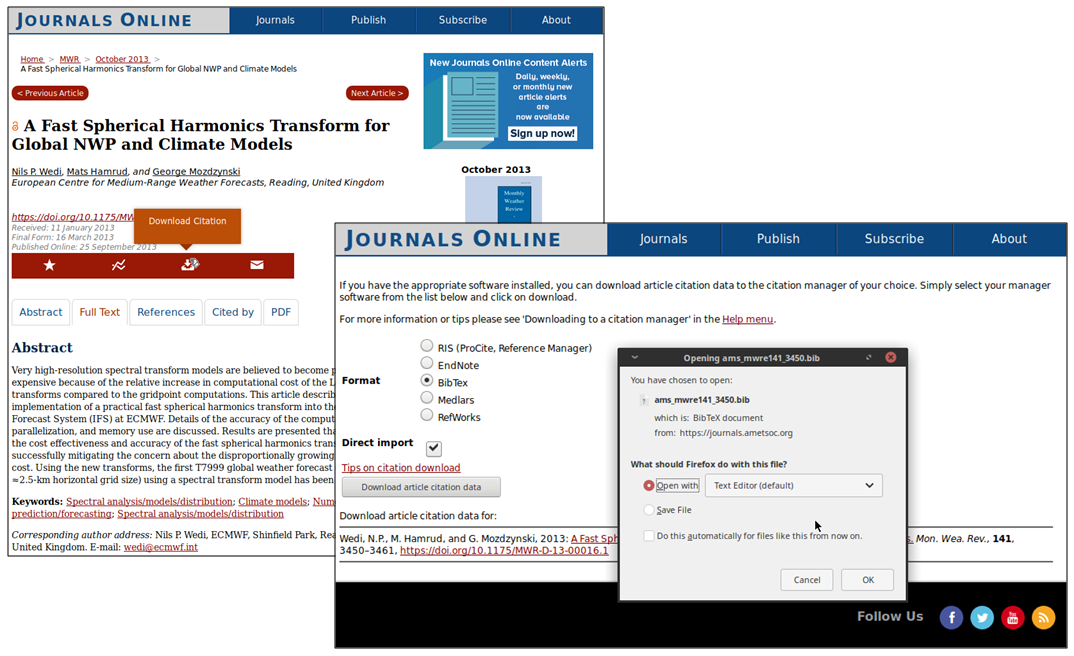
\includegraphics[scale=0.4]{./figs/exemplo_revista_ams_citacao.png}
    \caption{Download do arquivo de referência no formato BibTeX a partir da revista \textit{Monthly Weather Review} da \textit{American Meteorological Society}.}
    \label{fig:exemplo_revista_ams_citacao}
\end{figure}

No exemplo da Figura \ref{fig:exemplo_revista_ams_citacao}, o conteúdo do arquivo com a referência é mostrado a seguir:

%\begin{tcboxedraster}[raster columns=3, raster equal height, size=small,colframe=red!50!black,colback=red!10!white,colbacktitle=red!50!white, title={Box \# \thetcbrasternum}]{colback=yellow!10,fonttitle=\bfseries,title=Exemplo de um arquivo de referência no formato BibTeX}
\begin{texexp}{listing only}
@article{doi:10.1175/MWR-D-13-00016.1,
author   = {Wedi, Nils P. and Hamrud, Mats and Mozdzynski, George},
title    = {A Fast Spherical Harmonics Transform for Global NWP and Climate Models},
journal  = {Monthly Weather Review},
volume   = {141},
number   = {10},
pages    = {3450-3461},
year     = {2013},
doi      = {10.1175/MWR-D-13-00016.1},
URL      = {https://doi.org/10.1175/MWR-D-13-00016.1},
eprint   = {https://doi.org/10.1175/MWR-D-13-00016.1},
abstract = { AbstractVery high-resolution spectral transform models are believed to become prohibitively expensive because of the relative increase in computational cost of the Legendre transforms compared to the gridpoint computations. This article describes the implementation of a practical fast spherical harmonics transform into the Integrated Forecast System (IFS) at ECMWF. Details of the accuracy of the computations, of the parallelization, and memory use are discussed. Results are presented that demonstrate the cost effectiveness and accuracy of the fast spherical harmonics transform, successfully mitigating the concern about the disproportionally growing computational cost. Using the new transforms, the first T7999 global weather forecast (equivalent to ≈2.5-km horizontal grid size) using a spectral transform model has been produced.}
}
\end{texexp}

As informações do arquivo de referência baixado, podem ser incorporadas em uma seção apropriada no documento que o usuário estiver editando. No caso do estilo do INPE, o conteúdo do arquivo pode ser copiado para dentro do arquivo {\tt bib/referencias.bib}.

Observe que o arquivo de referências possui diversas palavras-chave, como por exemplo, {\tt author}, {\tt title}, {\tt journal}, {\tt volume} e outros. Estas são as informações que o BibTeX utiliza para formatar a apresentação das referências no estilo desejado.

\begin{marker}
  É uma boa ideia alterar o nome da citação (a qual será usada no texto) para algo que seja mais fácil de lembrar. Isso facilitará a escrita do texto. Por exemplo, ao invés de utilizar {\tt doi:10.1175/MWR-D-13-00016.1} (como na referência do exemplo acima), utilize algo como {\tt wedietal/2013}, que faz referência literal ao artigo de \citeonline{doi:10.1175/MWR-D-13-00016.1}.
\end{marker}

A utilização das referências no texto deve ser feita com os seguintes comandos: {\tt cite} ou {\tt citeonline}. Veja o Exemplo \ref{exe:ref2} a seguir:

\begin{texexptitled}[breakable,center lower,enhanced,middle=2mm]{Exemplos de citações utilizando os comandos {\tt cite} e {\tt citeonline}}{exe:ref2}
Segundo \citeonline{wedietal/2013}, a transformada rápida de Legendre torna-se especialmente útil em modelos espectrais cujo número de onda seja maior do que 2047.

A transformada rápida de Legendre torna-se especialmente útil em modelos espectrais cujo número de onda seja maior do que 2047 \cite{wedietal/2013}.
\end{texexptitled}

No Exemplo \ref{exe:ref2}, observe que o comando {\tt cite} marca a citação com a primeira letra em caixa alta, enquanto que com o comando {\tt citeonline}, a citação aparece delimitada por parênteses e com todas as letras em caixa alta. 

% REF: https://texblog.org/2012/10/22/multiple-bibliographies-with-biblatex/

%\begin{texexptitled}[breakable,center lower,enhanced,middle=2mm]{Exemplos de estilos de referências do BibTeX}{exe_estilos_bib}
%Segundo \cite{doi:10.1175/MWR-D-13-00016.1}, a transformada rápida de Legendre torna-se especialmente útil em modelos espectrais cujo número de onda seja maior do que 2047.
%
%\bibliographystyle{abbrv}
%\bibliography{./bib/referencia}
%
%\cite{doi:10.1175/MWR-D-13-00016.1} and \cite{doi:10.1175/MWR-D-13-00016.1} were published later than \citeNew{doi:10.1175/MWR-D-13-00016.1}.
%
%\bibliographystyle{plain}
%\bibliography{./bib/referencia}
%
%\bibliographystyleNew{plain}
%\bibliographyNew{./bib/referencia}
%\end{texexptitled}

\begin{marker}
  Deve-se ter cautela na edição manual do arquivo {\tt referencia.bib} do estilo do INPE. Este arquivo não aceita acentos naturais, i.e., acentos latinos devem ser marcados no estilo do LaTeX (veja mais detalhes na Seção \ref{sec:acentos}. Além disso, é recomendável que o usuário edite a referência, removendo espaços em brancos e remarcando os acentos, quando necessário.
\end{marker}

\subsubsection*{Estilos de Referências}
\label{sec:estilos_refs}

É possível utilizar diferentes estilos de referências. No estilo do INPE, utiliza-se o modelo da ABNT, que é provido a partir da utilização do pacote {\tt abntex2} (carregado automaticamente com o estilo do INPE). Em um documento livre, o usuário pode escolher outros estilos. Para isto, basta utilizar o comando \mintinline{latex}{\bibliographystyle}, indicando-se o estilo como argumento do marcador.

\subsubsection*{Citações}
\label{sec:cita}

\subsubsection*{Bibliografia}
\label{sec:biblio}

Atualmente a maioria das revistas fornecem as referências em diferentes formatos. Se houver dificuldade em obter o formato BibTeX de uma referência, pode-se utilizar o site \href{https://doi2bib.org}{DOI2Bib} para se obter a referência com os campos corretos.

\subsubsection*{Referências cruzadas}
\label{sec:refs_cruz}

\subsubsection*{Índice remissivo}
\label{sec:ind_rem}

\subsubsection*{Glossário}
\label{sec:glossario}
%http://linorg.usp.br/CTAN/macros/latex/contrib/glossaries/glossaries-user.html#sec:lipsum

\subsection{Macros e Comandos}
\label{sec:mac_cmd}

No LaTeX é possível definir \textit{macros}, que são um conjunto de instruções específicas para facilitar a formatação do documento. Além das \textit{macros}, é possível também redefinir comando do LaTeX, de forma que os comandos originais sejam executados de forma mais simples e customizada.

% Exemplo: redefinir o comando arraystretch de forma que a distância entre as linhas seja sempre um pouco maior (em comparação com o original): \renewcommand{\arraystretch}{1.2}

\subsection{Editores}
\label{sec:editores}

Muitos editores podem ser utilizados para editar documentos LaTeX. A escolha de um editor é particular, mas pode ser associada à forma como o usuário está mais habituado a digitar. Por exemplo, se o usuário gosta de utilizar o editor \href{https://www.vim.org}{VIM}, pode escolher instalar algumas extensões para este editor, a fim de torná-lo apto para a edição de documentos LaTeX. Outras escolhas de editores, podem incluir editores locais (como o próprio VIM, disponível para o Windows, Linux e Mac OS X) ou editores online. Editores locais podem variar de acordo com o sistema operacional em uso, embora muitos projetos \textit{open source} tenham executáveis para os sistemas operacionais mais utilizados. Em relação aos editores online, estes podem ser mais vantajosos por não dependerem do tipo de sistema operacional, mas apenas de uma conexão com a internet e um navegador compatível. Outra vantagem dos editores online, é o fato de que estes podem ser integrados a outros serviços, como o \href{https://dropbox.com}{Dropbox}.

Nas duas seções a seguir, são apresentados alguns editores selecionados para a edição de documentos LaTeX.

\subsubsection*{Editores locais}
\label{sec:ed_local}

Para compilar um documento LaTeX localmente, dependendo do sistema operacional em uso, há várias opções de editores. Por simplicidade, iremos escolher o editor TexMaker, disponível para os sistemas operacional \textit{Windows}, Linux e Mac OS.

Se a escolha do usuário for a linha de comando, utilizando um editor como o VIM, os documentos em LaTeX podem ser compilados utilizando uma sequência de comandos como a seguir:

No caso do estilo do INPE para teses, dissertações e relatórios (mais detalhes no Caítulo \ref{cap:parteIII}), pode-se utilizar o \textit{script} {\tt execpub.sh} para facilitar o processo de compilação. O que este \textit{script} faz é executar a sequência de comando do exemplo anterior, realizando mais alguns procedimentos para a renderização correta das referências com o estilo do INPE. 

\begin{marker}
  Veja o \href{http://mtc-m16d.sid.inpe.br/col/sid.inpe.br/mtc-m19@80/2010/03.24.15.12/doc/ambiente_latex_no_linux.pdf}{documento} para mais detalhes sobre a utilização do \textit{script} {\tt execpub.sh}.
\end{marker}

\subsubsection*{Editores online}
\label{sec:ed_online}

O Overleaf é um editor LaTeX online que pode ser utilizado para escrita colaborativa. O estilo do INPE está disponível na plataforma online e pode ser carregado para a escrita de teses e dissertações a partir de endereço \url{https://www.overleaf.com/latex/templates/inpe-thesis-template/scdyfqzhbycc#.Wrj8gH8h2Uk}. Para acessar, é necessário que o usuário crie uma conta para o acesso. Esta é a forma recomendada para a criação de documentos LaTeX, especialmente se o usuário ainda não está familiarizado com documentos mais complexos como o estilo do INPE.

%\begin{dica}{Dica \#3}
%  Ao utilizar o Overleaf, você irá perceber que a compilação do documento pode levar mais tempo quando muitas figuras são incluídas. Experimente comentar as seções do texto que já foram revistas para acelerar a compilação.
%\end{dica}
\begin{marker}
  Ao utilizar o Overleaf, você irá perceber que a compilação do documento pode levar mais tempo quando muitas figuras são incluídas. Experimente comentar as seções do texto que já foram revistas para acelerar a compilação.
\end{marker}

%\begin{tcbitemize}[raster columns=4,raster rows=4,raster height=0.8\linewidth,raster every box/.style={size=small,beamer,colframe=blue!75!yellow,colback=red!75!yellow!20,center title,title=Box}]
%\tcbitem One
%\tcbitem Two
%\tcbitem Three
%\tcbitem Four
%\tcbitem[raster multirow=2,blankest]
%\begin{tcbitemize}[raster columns=1,raster rows=2,raster height=\tcbtextheight]
%\tcbitem Twelve
%\tcbitem Eleven
%\end{tcbitemize}
%\tcbitem[raster multirow=2,raster multicolumn=2,colframe=red!75!yellow,colback=blue!75!yellow!20]This is an example with fixed height boxes.
%\tcbitem[raster multirow=2,blankest]
%\begin{tcbitemize}[raster columns=1,raster rows=2,raster height=\tcbtextheight]
%\tcbitem Five
%\tcbitem Six
%\end{tcbitemize}
%\tcbitem Ten
%\tcbitem Nine
%\tcbitem Eight
%\tcbitem Seven
%\end{tcbitemize}
%
%\begin{tcbitemize}
%[raster columns=2,raster rows=1,raster height=0.8\linewidth,raster every box/.style={size=small,beamer,colframe=blue!75!yellow,colback=red!75!yellow!20,center title,title=Box}]
%\tcbitem One
%    fff
%\tcbitem Two
%dsfsdf
%\end{tcbitemize}
%
%\begin{tcbitemize}[raster equal height=rows,raster columns=3,title=\thetcbrasternum,colframe=red!50!black,colback=red!10!white]\tcbitem[colframe=blue!50!black,colback=blue!10!white,raster multicolumn=1]multicolumn=1
%\tcbitem
%\tcbitem
%\tcbitem[colframe=blue!50!black,colback=blue!10!white,raster multicolumn=2]multicolumn=2\tcbitem\tcbitem[colframe=blue!50!black,colback=blue!10!white,raster multicolumn=3]multicolumn=3\tcbitem\tcbitem[colframe=blue!50!black,colback=blue!10!white,raster multicolumn=2]multicolumn=2\end{tcbitemize}

\section{Exercícios}
\label{sec:exercicios}

Para colocar em prática os comandos de marcação do $\LaTeX$, realize os exercícios a seguir. As respostas estão no Anexo \ref{anexoA}. Cada exercício contém um link para o anexo, que irá lhe direcionar para a resposta correta. Para fazer os exercícios, você pode utilizar um editor local (instalado em seu computador) ou um editor online, como o \href{https://pt.overleaf.com/project}{Overleaf}.

Para a realização dos exercícios, utilize os exemplos dados ao longo das seções do Capítulo \ref{cap:parteII}. Utilize também as tabelas do Anexo \ref{anexoB}.

\tcbstartrecording

\subsection*{Marcação de Texto}
\label{sec:exec_mar_text}

Os exercícios a seguir mostram como formatar texto utilizando as marcações mais comuns mostradas na Seção \ref{sec:marc_text}.

\begin{texercise}{Ex1}\textit{Formate a frase abaixo utilizando os estilos \mintinline{latex}{\textbf}, \mintinline{latex}{\underline} e \mintinline{latex}{\textit}}:\par\smallskip%
\begin{tcboutputlisting}
\begin{center}
    The \textbf{brown} fox \underline{jumps} over the \textit{lazy} dog.
\end{center}
\end{tcboutputlisting}
\tcbuselistingtext%
\end{texercise}

\subsection*{Listas}
\label{sec:exec_listas}

\begin{texercise}{Ex2}\textit{Marque as palavras da frase abaixo usando os estilos visíveis}:\par\smallskip%
\begin{tcboutputlisting}
\begin{center}
    The \textbf{brown} fox \underline{jumps} over the \textit{lazy} dog.
\end{center}
\end{tcboutputlisting}
\tcbuselistingtext%
\end{texercise}

\subsection*{Tabelas}
\label{sec:exec_tabelas}

\begin{texercise}{Ex3}\textit{Crie a seguinte tabela:}\par\smallskip%
\begin{tcboutputlisting}
\begin{tabular}{|p{3cm}|p{3cm}|p{3cm}|p{3cm}|}\hline
\multicolumn{4}{|c|}{\bfseries\itshape Das alte Italien}\\\hline
\multicolumn{2}{|c|}{\bfseries Antike} &
\multicolumn{2}{c|}{\bfseries Mittelalter}\\\hline
\multicolumn{1}{|c|}{\itshape Republik}&
\multicolumn{1}{c|}{\itshape Kaiserreich}&
\multicolumn{1}{c|}{\itshape Franken}&
\multicolumn{1}{c|}{\itshape Teilstaaten}\\\hline
In den Zeiten der r\"{o}mischen Republik standen dem Staat jeweils zweiKonsuln vor, deren Machtbefugnisse identisch waren. &
Das r\"{o}mische Kaiserreich wurde von einem Alleinherrscher, dem Kaiser,regiert.& 
In der V\"{o}lkerwanderungszeit \"{u}bernahmen die Goten und sp\"{a}ter dieFranken die Vorherrschaft.& 
Im sp\"{a}teren Mittelalter regierten F\"{u}rsten einen Fleckenteppichvon Einzelstaaten.\\\hline
\end{tabular}
\end{tcboutputlisting}
\tcbuselistingtext%
\end{texercise}

\subsection*{Macros com 1 parâmetro}
\label{sec:exec_macros_1_par}

\begin{texercise}{Ex4}
\begin{tcboutputlisting}
\newcommand{\headingline}[1]{%
    \begin{center}\Large\bfseries #1\end{center}}
\end{tcboutputlisting}
\tcbuselistingtext%
Crie uma nova macro \verb+\headingline+ que produza o seguinte resultado:\par\smallskip
\begin{tcbwritetemp}
\headingline{Título muito importante}
\end{tcbwritetemp}\tcbusetemplisting\tcbusetemp%
\end{texercise}

\subsection*{Macros com 2 parâmetros}
\label{sec:exec_macros_2_par}

\begin{texercise}{Ex5}
\begin{tcboutputlisting}
\newcommand{\minitable}[2]{%
    \begin{center}\begin{tabular}{p{10cm}}\hline%
    \multicolumn{1}{c}{\bfseries#1}\\\hline%
    #2\\\hline%
    \end{tabular}\end{center}}
    \end{tcboutputlisting}
    \tcbuselistingtext%
    Crie uma nova macro \verb+\minitable+ que produza o seguinte resultado:\par\smallskip\begin{tcbwritetemp}
    \minitable{Meu título}{Nesta pequena tabela, há apenas um título e algum texto abaixo com largura de dez centímetros.}
    \end{tcbwritetemp}
    \tcbusetemplisting\par\smallskip\tcbusetemp%
\end{texercise}

\subsection*{Matemática e Equações}
\label{sec:exec_mat_eqs}

\begin{texercise}{Ex_Eq1}\textit{Crie uma matriz sem delimitadores}:\par\smallskip%
\begin{tcboutputlisting}
    \begin{center}
        \begin{equation*}
            \begin{matrix} 
                a & b \\ 
                c & d 
            \end{matrix}
        \end{equation*}
    \end{center}
\end{tcboutputlisting}
\tcbuselistingtext%
\end{texercise}

\begin{texercise}{Ex_Eq2}\textit{Crie uma matriz com delimitadores quadrados}:\par\smallskip%
\begin{tcboutputlisting}
    \begin{center}
        \begin{equation*}
            \begin{bmatrix} 
                1 & 2 & -1 \\ 
                3 & 0 & 1 \\ 
                0 & 2 & 4 
            \end{bmatrix}
        \end{equation*}
    \end{center}
\end{tcboutputlisting}
\tcbuselistingtext%
\end{texercise}

\begin{texercise}{Ex_Eq3}\textit{Utilize \mintinline{latex}{(} e \mintinline{latex}{)} para delimitar uma expressão arbitrária entre parênteses}:\par\smallskip%
\begin{tcboutputlisting}
    \begin{center}
        \begin{equation*}
            \left( \frac{p}{q} \right)
        \end{equation*}
    \end{center}
\end{tcboutputlisting}
\tcbuselistingtext%
\end{texercise}

\begin{texercise}{Ex_Eq4}\textit{A derivada \(f'(a)\) da função \(f(x)\) no ponto \(x=a\) é o limite}:\par\smallskip%
\begin{tcboutputlisting}
    \begin{center}
        \begin{equation*}
            f'(a) = \lim_{x \to a} \frac{f(x) - f(a)}{x - a}
        \end{equation*}
    \end{center}
\end{tcboutputlisting}
\tcbuselistingtext%
\end{texercise}

\begin{texercise}{Ex_Eq5}\textit{A função \(f(x)\) é contínua no ponto \(x=a\) se}:\par\smallskip%
\begin{tcboutputlisting}
    \begin{center}
        \begin{equation*}
            \lim_{x \to a^-} f(x) = f(a) = \lim_{x \to a^+} f(x)
        \end{equation*}
    \end{center}
\end{tcboutputlisting}
\tcbuselistingtext%
\end{texercise}

\begin{texercise}{Ex_Eq6}\textit{A série de MacLaurin para \(e^x\) é}:\par\smallskip%
\begin{tcboutputlisting}
    \begin{center}
        \begin{equation*}
            e^x = \sum_{k=0}^{\infty} \frac{x^k}{k!}
        \end{equation*}
    \end{center}
\end{tcboutputlisting}
\tcbuselistingtext%
\end{texercise}

\begin{texercise}{Ex_Eq7}\textit{A matriz Jacobiano da função \(\mathbf{f}(x_1, \dots, x_n)\) é}:\par\smallskip%
\begin{tcboutputlisting}
    \begin{center}
        \begin{equation*}
            \mathbf{J}
            =
            \frac{d \mathbf{f}}{d \mathbf{x}}
            =
            \left[ \frac{\partial \mathbf{f}}{\partial x_1}
            \cdots \frac{\partial \mathbf{f}}{\partial x_n} \right]
            =
            \begin{bmatrix}
            \frac{\partial f_1}{\partial x_1} & \cdots &
            \frac{\partial f_1}{\partial x_n} \\
            \vdots & \ddots & \vdots \\
            \frac{\partial f_m}{\partial x_1} & \cdots &
            \frac{\partial f_m}{\partial x_n}
            \end{bmatrix}
        \end{equation*}
    \end{center}
\end{tcboutputlisting}
\tcbuselistingtext%
\end{texercise}

\begin{texercise}{Ex_Eq8}\textit{Escreva um código LaTeX para mostrar a identidade da soma de dois ângulos}:\par\smallskip%
\begin{tcboutputlisting}
    \begin{center}
        \begin{equation*}
            \text{cos}(\alpha \pm \beta) = \text{cos}\alpha \text{cos}\beta \mp \text{sin}\alpha \text{sin}\beta
        \end{equation*}
    \end{center}
\end{tcboutputlisting}
\tcbuselistingtext%
\end{texercise}

\begin{texercise}{Ex_Eq9}\textit{Escreva um código LaTeX para mostrar a integral indefinida}:\par\smallskip%
\begin{tcboutputlisting}
    \begin{center}
        \begin{equation*}
            \int \frac{1}{a+x^2}dx = \text{arctan} x + C
        \end{equation*}
    \end{center}
\end{tcboutputlisting}
\tcbuselistingtext%
\end{texercise}

\begin{texercise}{Ex_Eq10}\textit{Escreva um código LaTeX para mostrar a equação de Navier-Stokes para um fluxo incompressível}:\par\smallskip%
\begin{tcboutputlisting}
    \begin{center}
        \begin{equation*}
            \frac{\partial{\mathbf{u}}}{\partial{t}} + (\mathbf{u} \cdot \nabla)\mathbf{u} - \nu \nabla^2 \mathbf{u} = - \nabla \omega + \mathbf{g}
        \end{equation*}
    \end{center}
\end{tcboutputlisting}
\tcbuselistingtext%
\end{texercise}

\begin{texercise}{Ex_Eq11}\textit{Escreva um código LaTeX para mostrar o Teorema de Green}:\par\smallskip%
\begin{tcboutputlisting}
    \begin{center}
        \begin{equation*}
            \oint_C (Ldx + Mdy) = \iint_D \bigg(\frac{\partial{M}}{\partial{x}} - \frac{\partial{L}}{\partial{y}}\bigg)dxdy
        \end{equation*}
    \end{center}
\end{tcboutputlisting}
\tcbuselistingtext%
\end{texercise}

\begin{texercise}{Ex_Eq12}\textit{Escreva um código LaTeX para mostrar o Teorema dos Números Primos}:\par\smallskip%
\begin{tcboutputlisting}
    \begin{center}
        \begin{equation*}
            \lim_{x \to \infty} \frac{\pi(x)}{\frac{x}{\text{log}(x)}} = 1
        \end{equation*}
    \end{center}
\end{tcboutputlisting}
\tcbuselistingtext%
\end{texercise}

\begin{texercise}{Ex_Eq13}\textit{Escreva um código LaTeX para mostrar a fórmula geral da série de Taylor}:\par\smallskip%
\begin{tcboutputlisting}
    \begin{center}
        \begin{equation*}
            \sum_{n=0}^{\infty} \frac{f^{(n)}(a)}{n!}(x-a)^n
        \end{equation*}
    \end{center}
\end{tcboutputlisting}
\tcbuselistingtext%
\end{texercise}

\begin{texercise}{Ex_Eq14}\textit{Escreva um código LaTeX para mostrar o Teorema de Stokes}:\par\smallskip%
\begin{tcboutputlisting}
    \begin{center}
        \begin{equation*}
            \int_{\partial{\Omega}} \omega = \int_{\Omega} d\omega
        \end{equation*}
    \end{center}
\end{tcboutputlisting}
\tcbuselistingtext%
\end{texercise}

\begin{texercise}{Ex_Eq15}\textit{Escreva um código LaTeX para mostrar a propriedade adjunta do produto tensorial}:\par\smallskip%
\begin{tcboutputlisting}
    \begin{center}
        \begin{equation*}
            \text{Hom}(U \otimes V, W) \cong \text{Hom}(U, \text{Hom}(V,W))
        \end{equation*}
    \end{center}
\end{tcboutputlisting}
\tcbuselistingtext%
\end{texercise}
  
\begin{texercise}{Ex_Eq16}\textit{Escreva um código LaTeX para mostrar a definição da transformada de Laplace}:\par\smallskip%
\begin{tcboutputlisting}
    \begin{center}
        \begin{equation*}
            \mathcal{L} \lbrace f(t) \rbrace = F(s) \int_{0}^{\infty} f(t) e^{-st} dt
        \end{equation*}
    \end{center}
\end{tcboutputlisting}
\tcbuselistingtext%
\end{texercise}
  
\begin{texercise}{Ex_Eq17}\textit{Escreva um código LaTeX para mostrar a fórmula da inversa de uma matriz}:\par\smallskip%
\begin{tcboutputlisting}
    \begin{center}
        \begin{equation*}
            \begin{bmatrix}
                a & b \\
                c & d \\
            \end{bmatrix}^{-1} 
            = \frac{1}{ad-bc} 
            \begin{bmatrix}
            d  & -b \\
            -c & a  \\
            \end{bmatrix}
        \end{equation*}
    \end{center}
\end{tcboutputlisting}
\tcbuselistingtext%
\end{texercise}
  
\begin{texercise}{Ex_Eq18}\textit{Escreva um código LaTeX para mostrar a fórmula do produto infinito}:\par\smallskip%
\begin{tcboutputlisting}
    \begin{center}
        \begin{equation*}
            \text{sin}x = x \prod^{\infty}_{n=1} \bigg(1 - \frac{x^2}{\pi^{2} n^{2}} \bigg)
        \end{equation*}
    \end{center}
\end{tcboutputlisting}
\tcbuselistingtext%
\end{texercise}
   
\tcbstoprecording